\begin{appendices}

\chapter{Ascending Filtration of the Contour Tree}
\label{chapter-asc}

\begin{figure}[h]%
    \captionsetup[subfigure]{labelformat=empty}
    \centering
    \subfloat[$CT(X)_0$]{{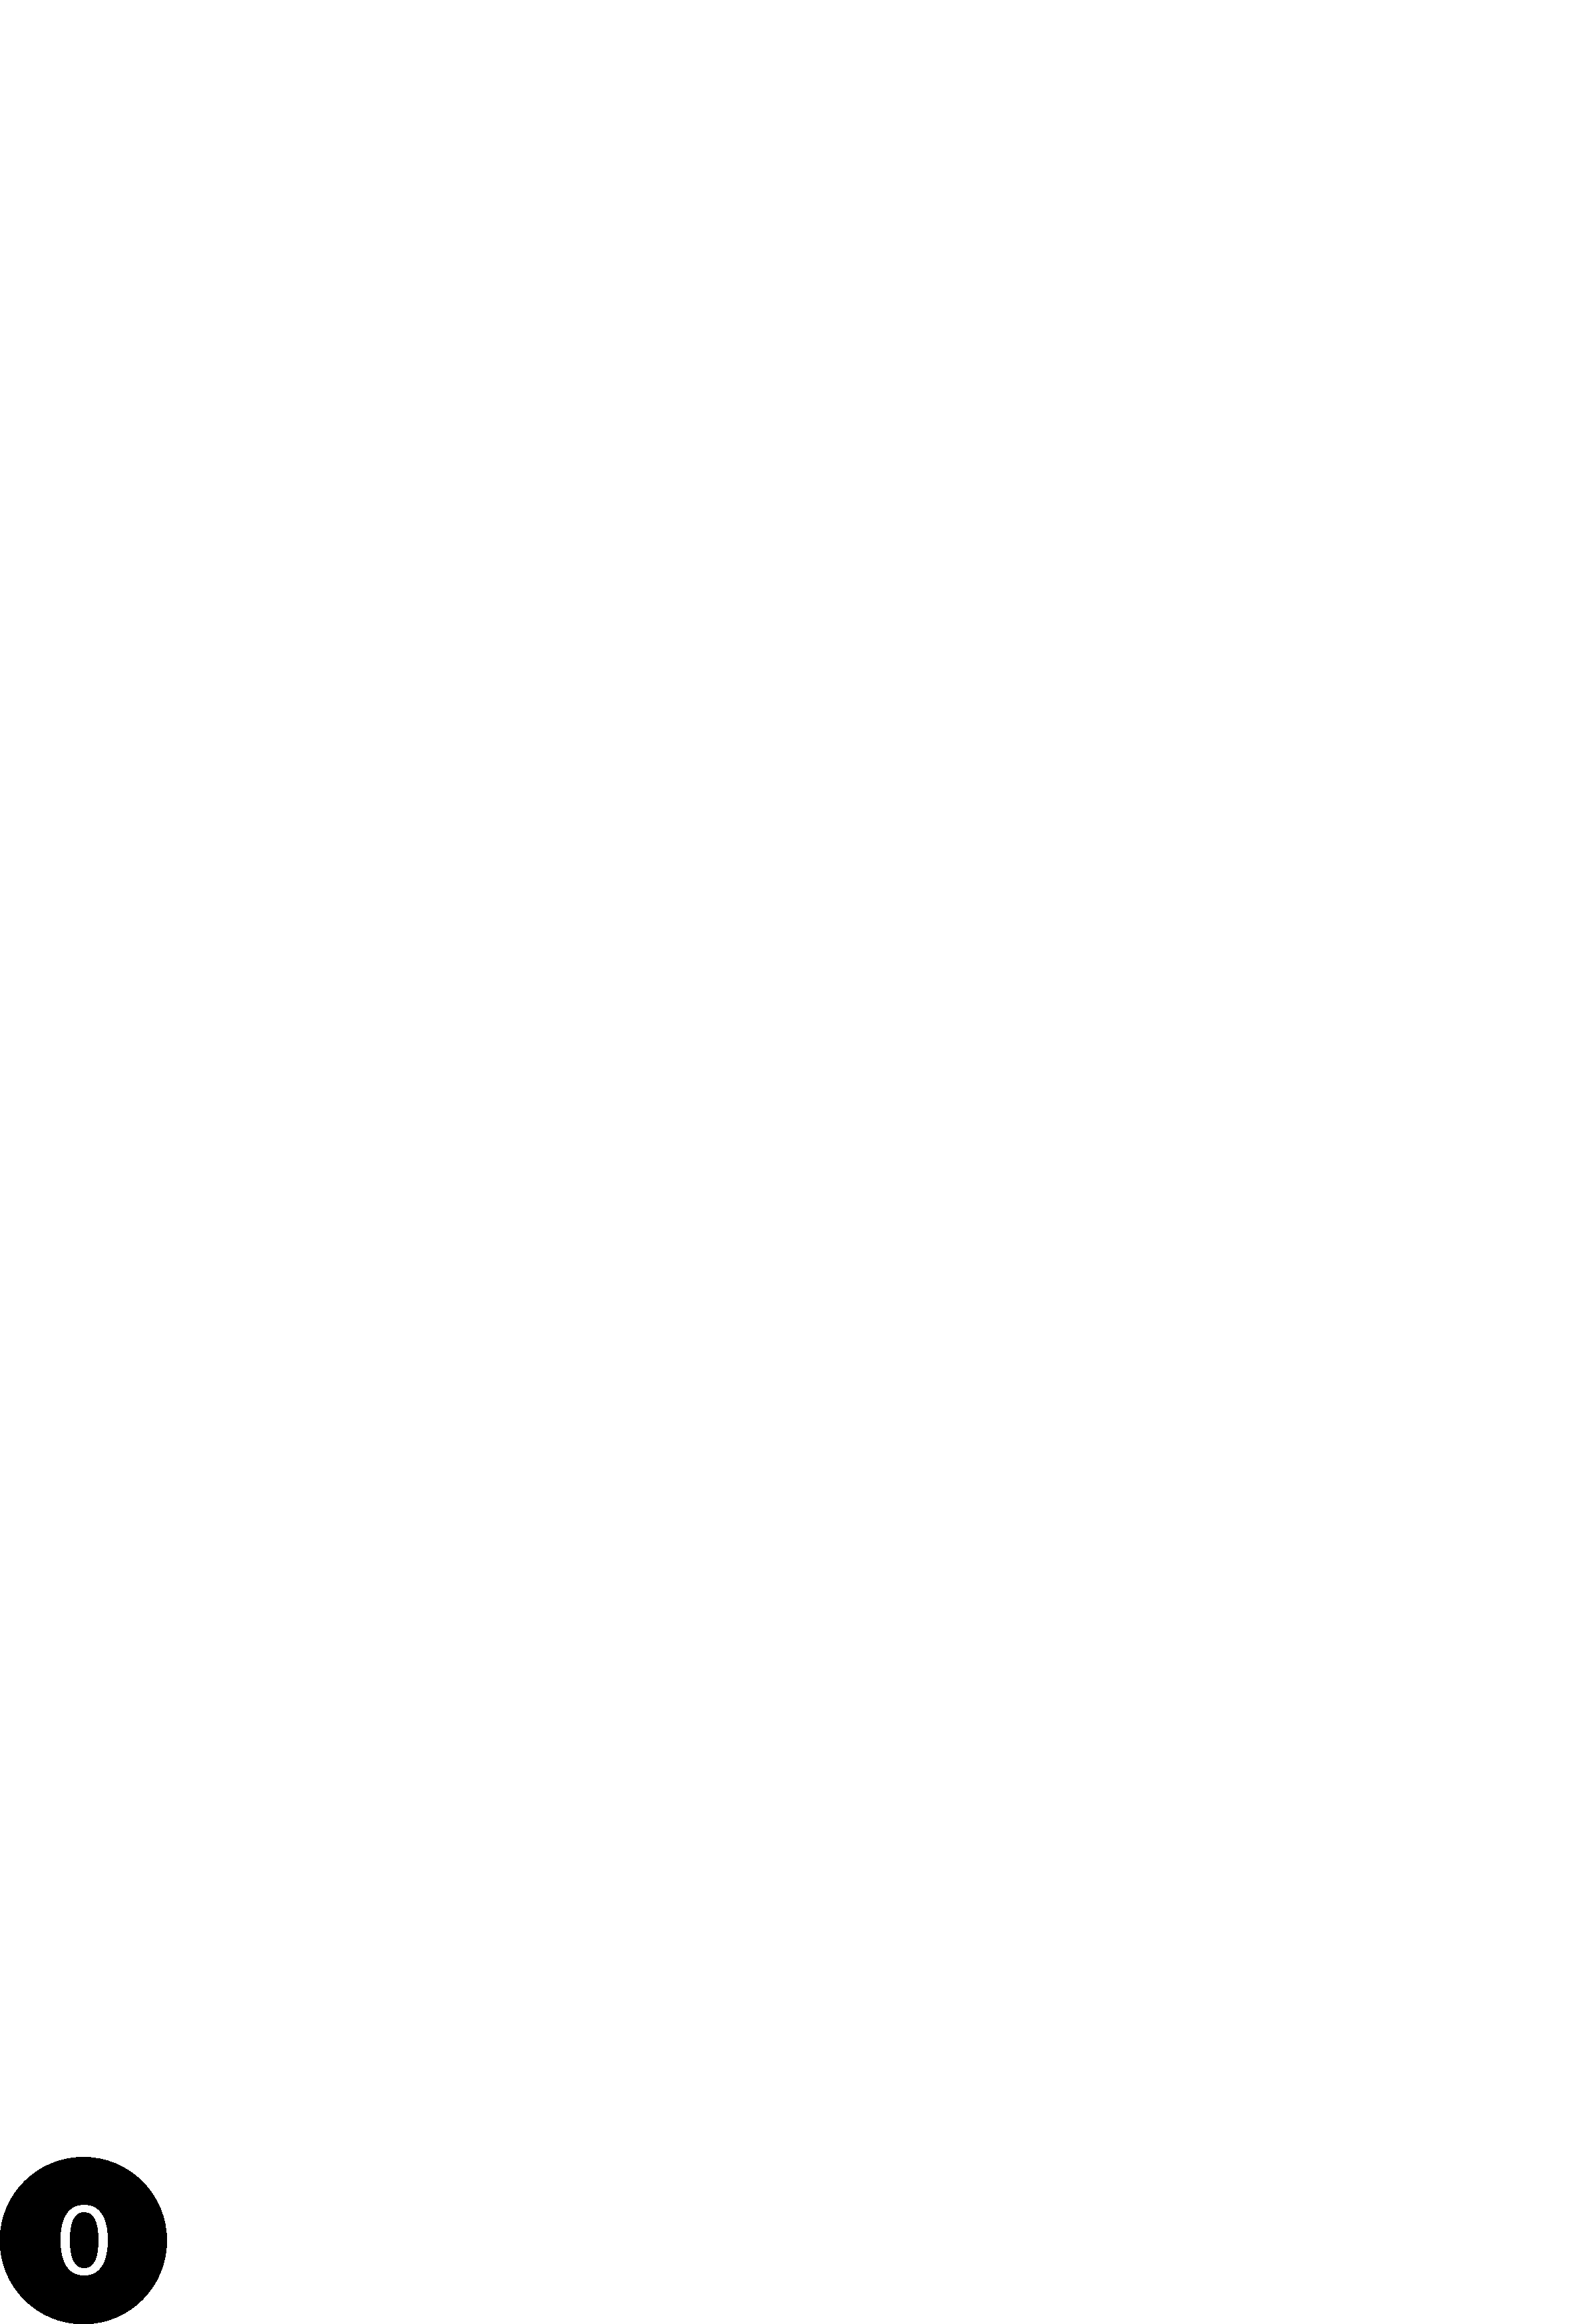
\includegraphics[scale=0.08]{./images/filtration/asc-tree/x1.pdf}}}%
    \qquad
    \subfloat[$CT(X)_1$]{{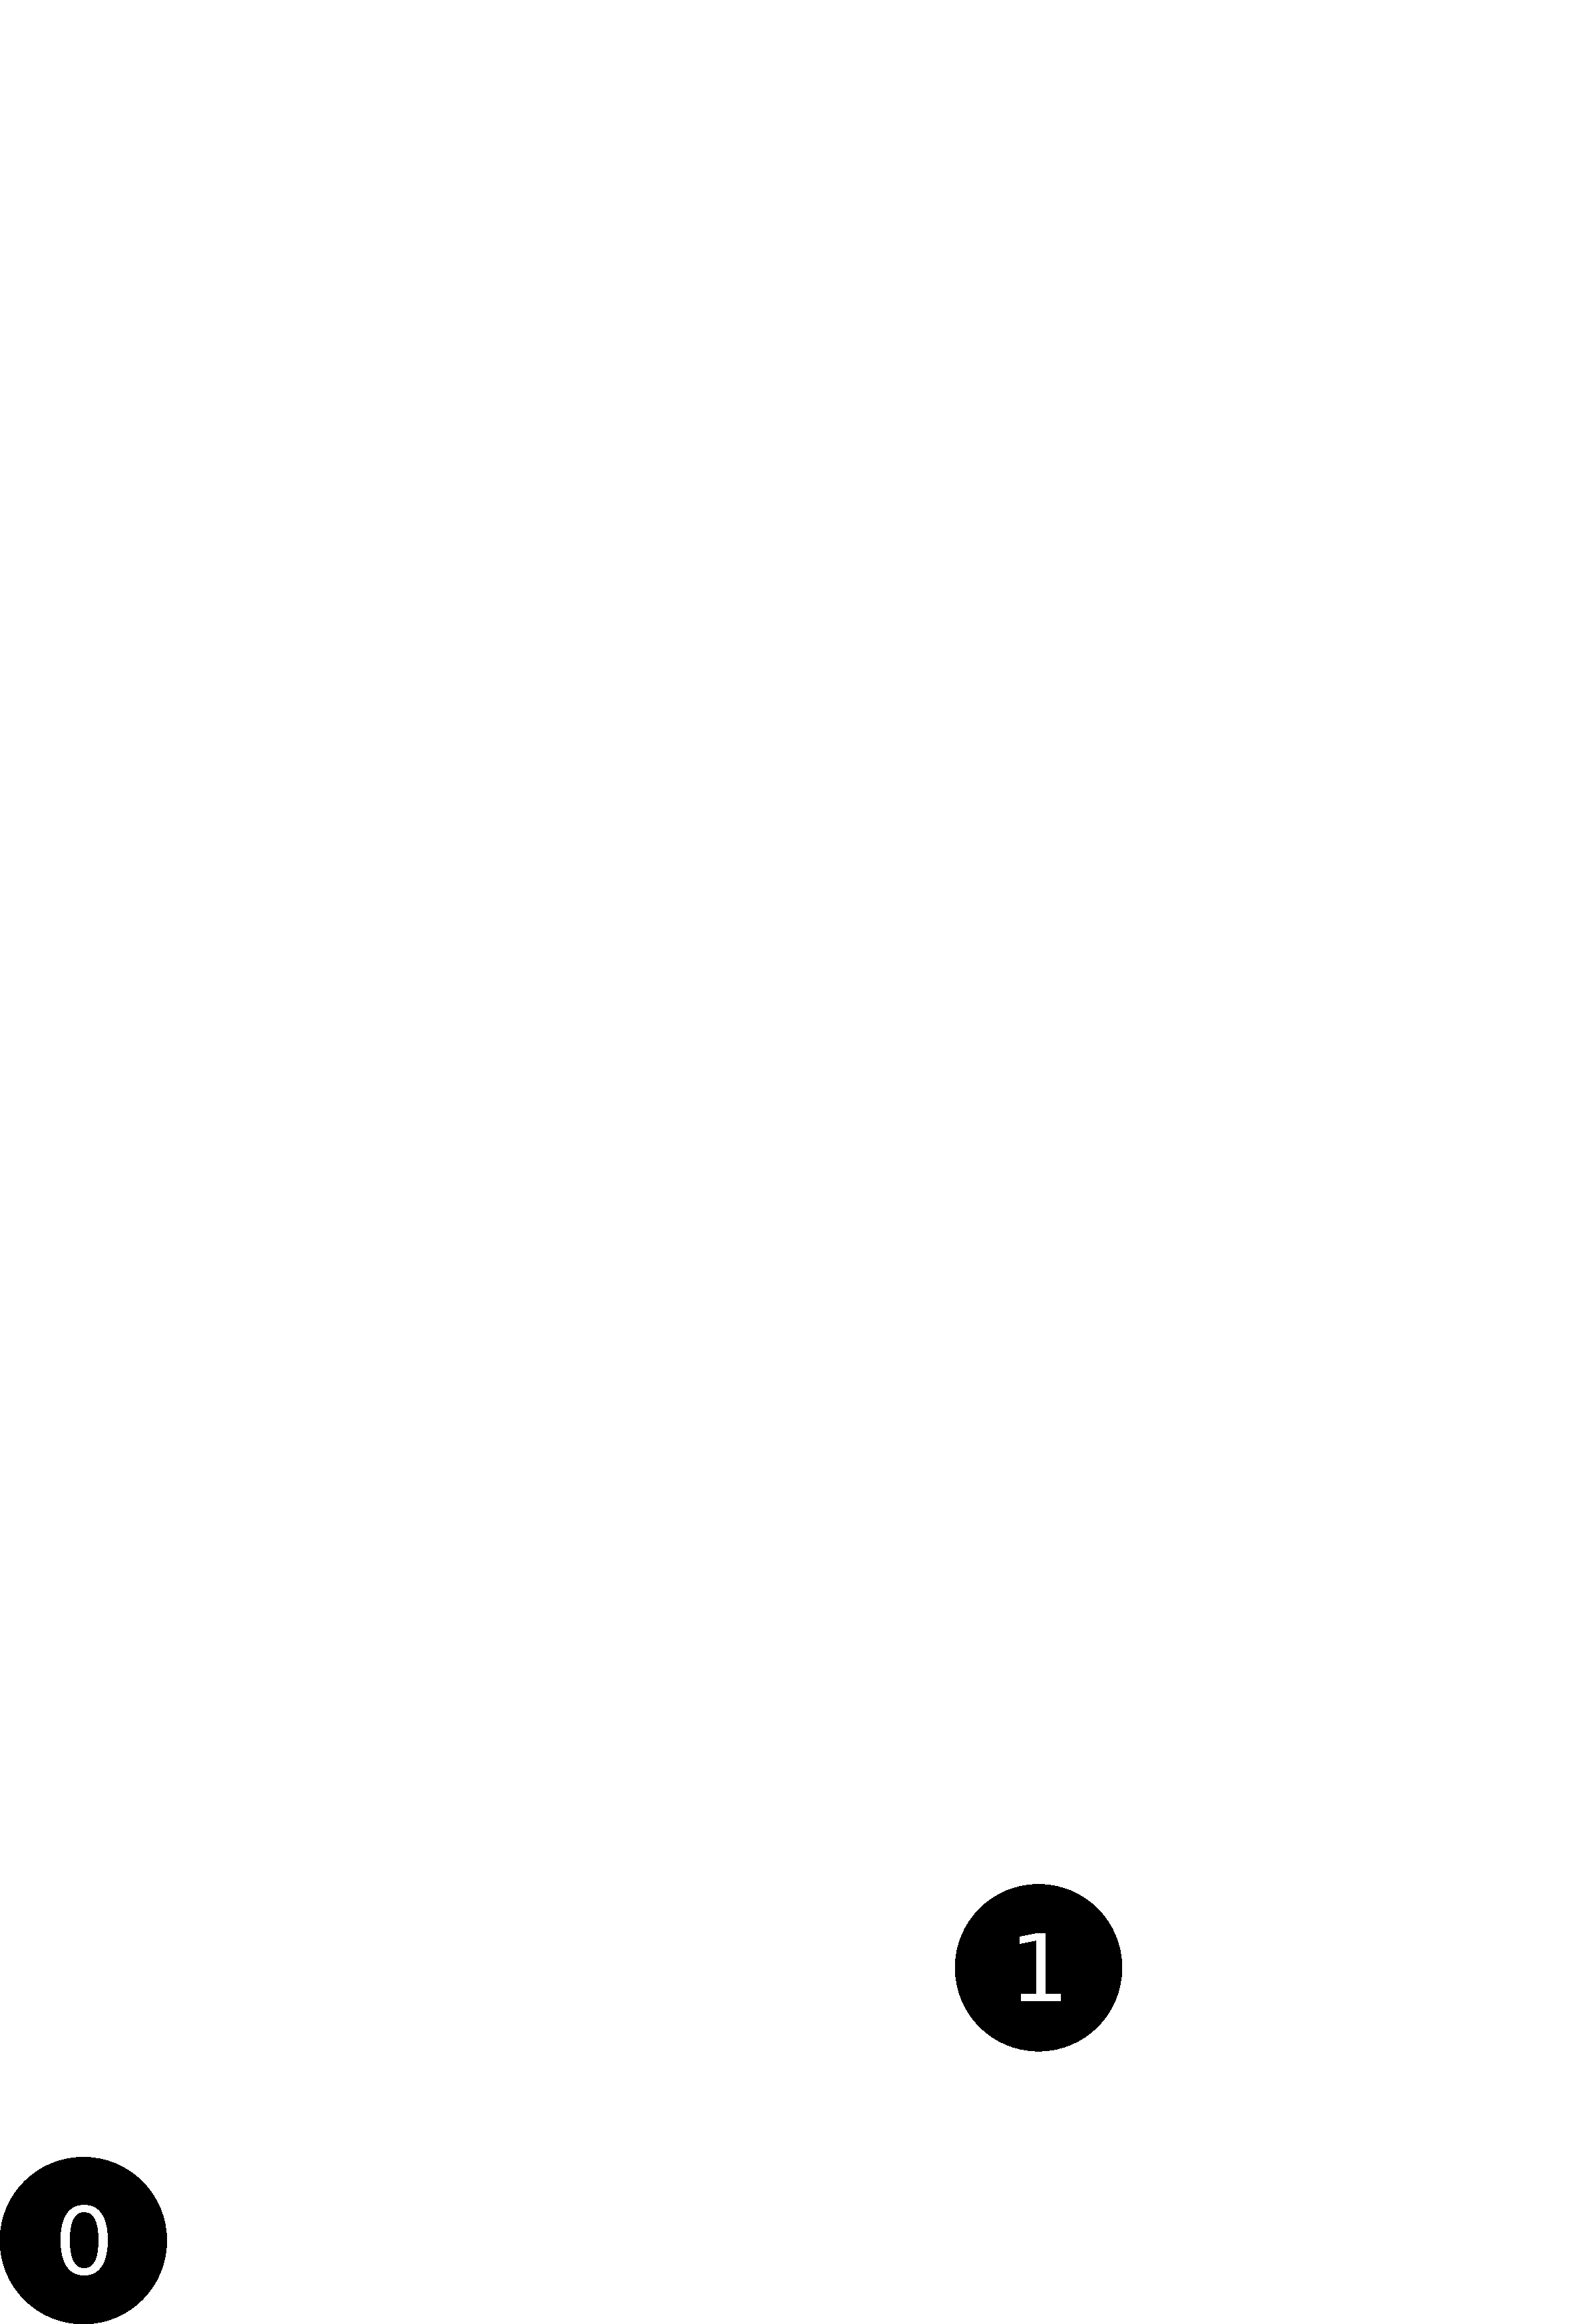
\includegraphics[scale=0.08]{./images/filtration/asc-tree/x2.pdf}}}%
    \qquad
    \subfloat[$CT(X)_2$]{{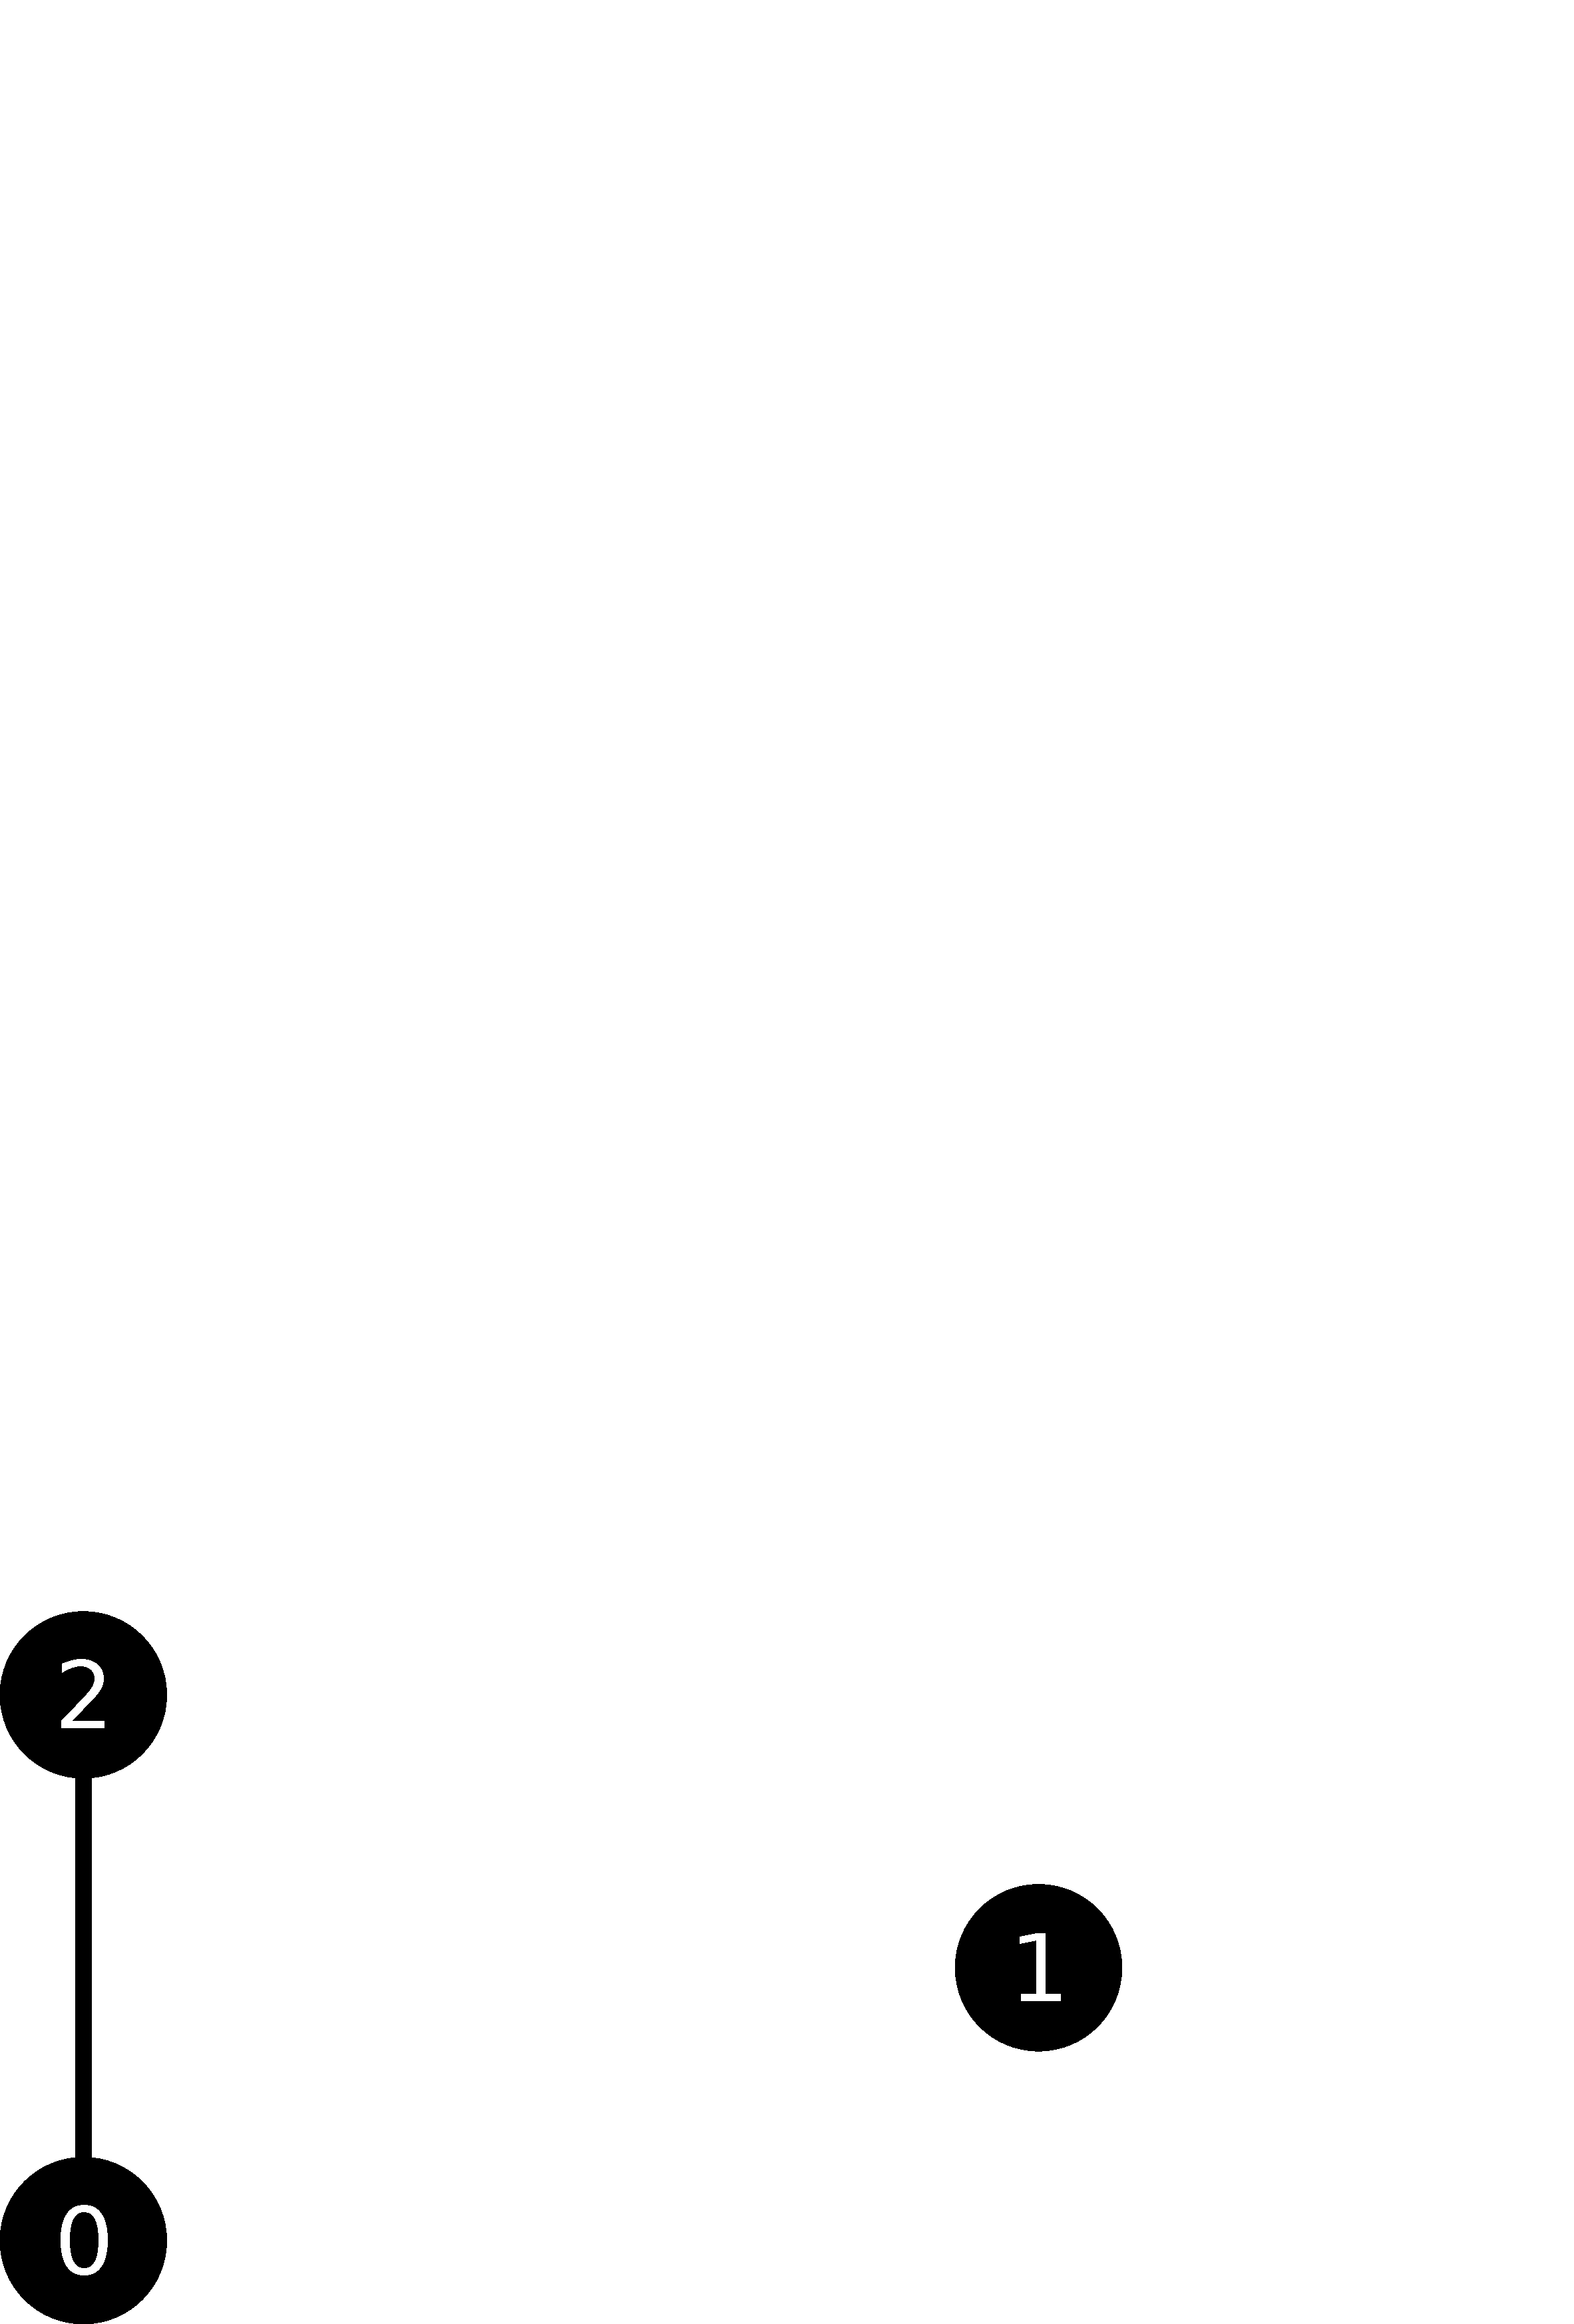
\includegraphics[scale=0.08]{./images/filtration/asc-tree/x3.pdf}}}%

    \par\bigskip

    \subfloat[$CT(X)_3$]{{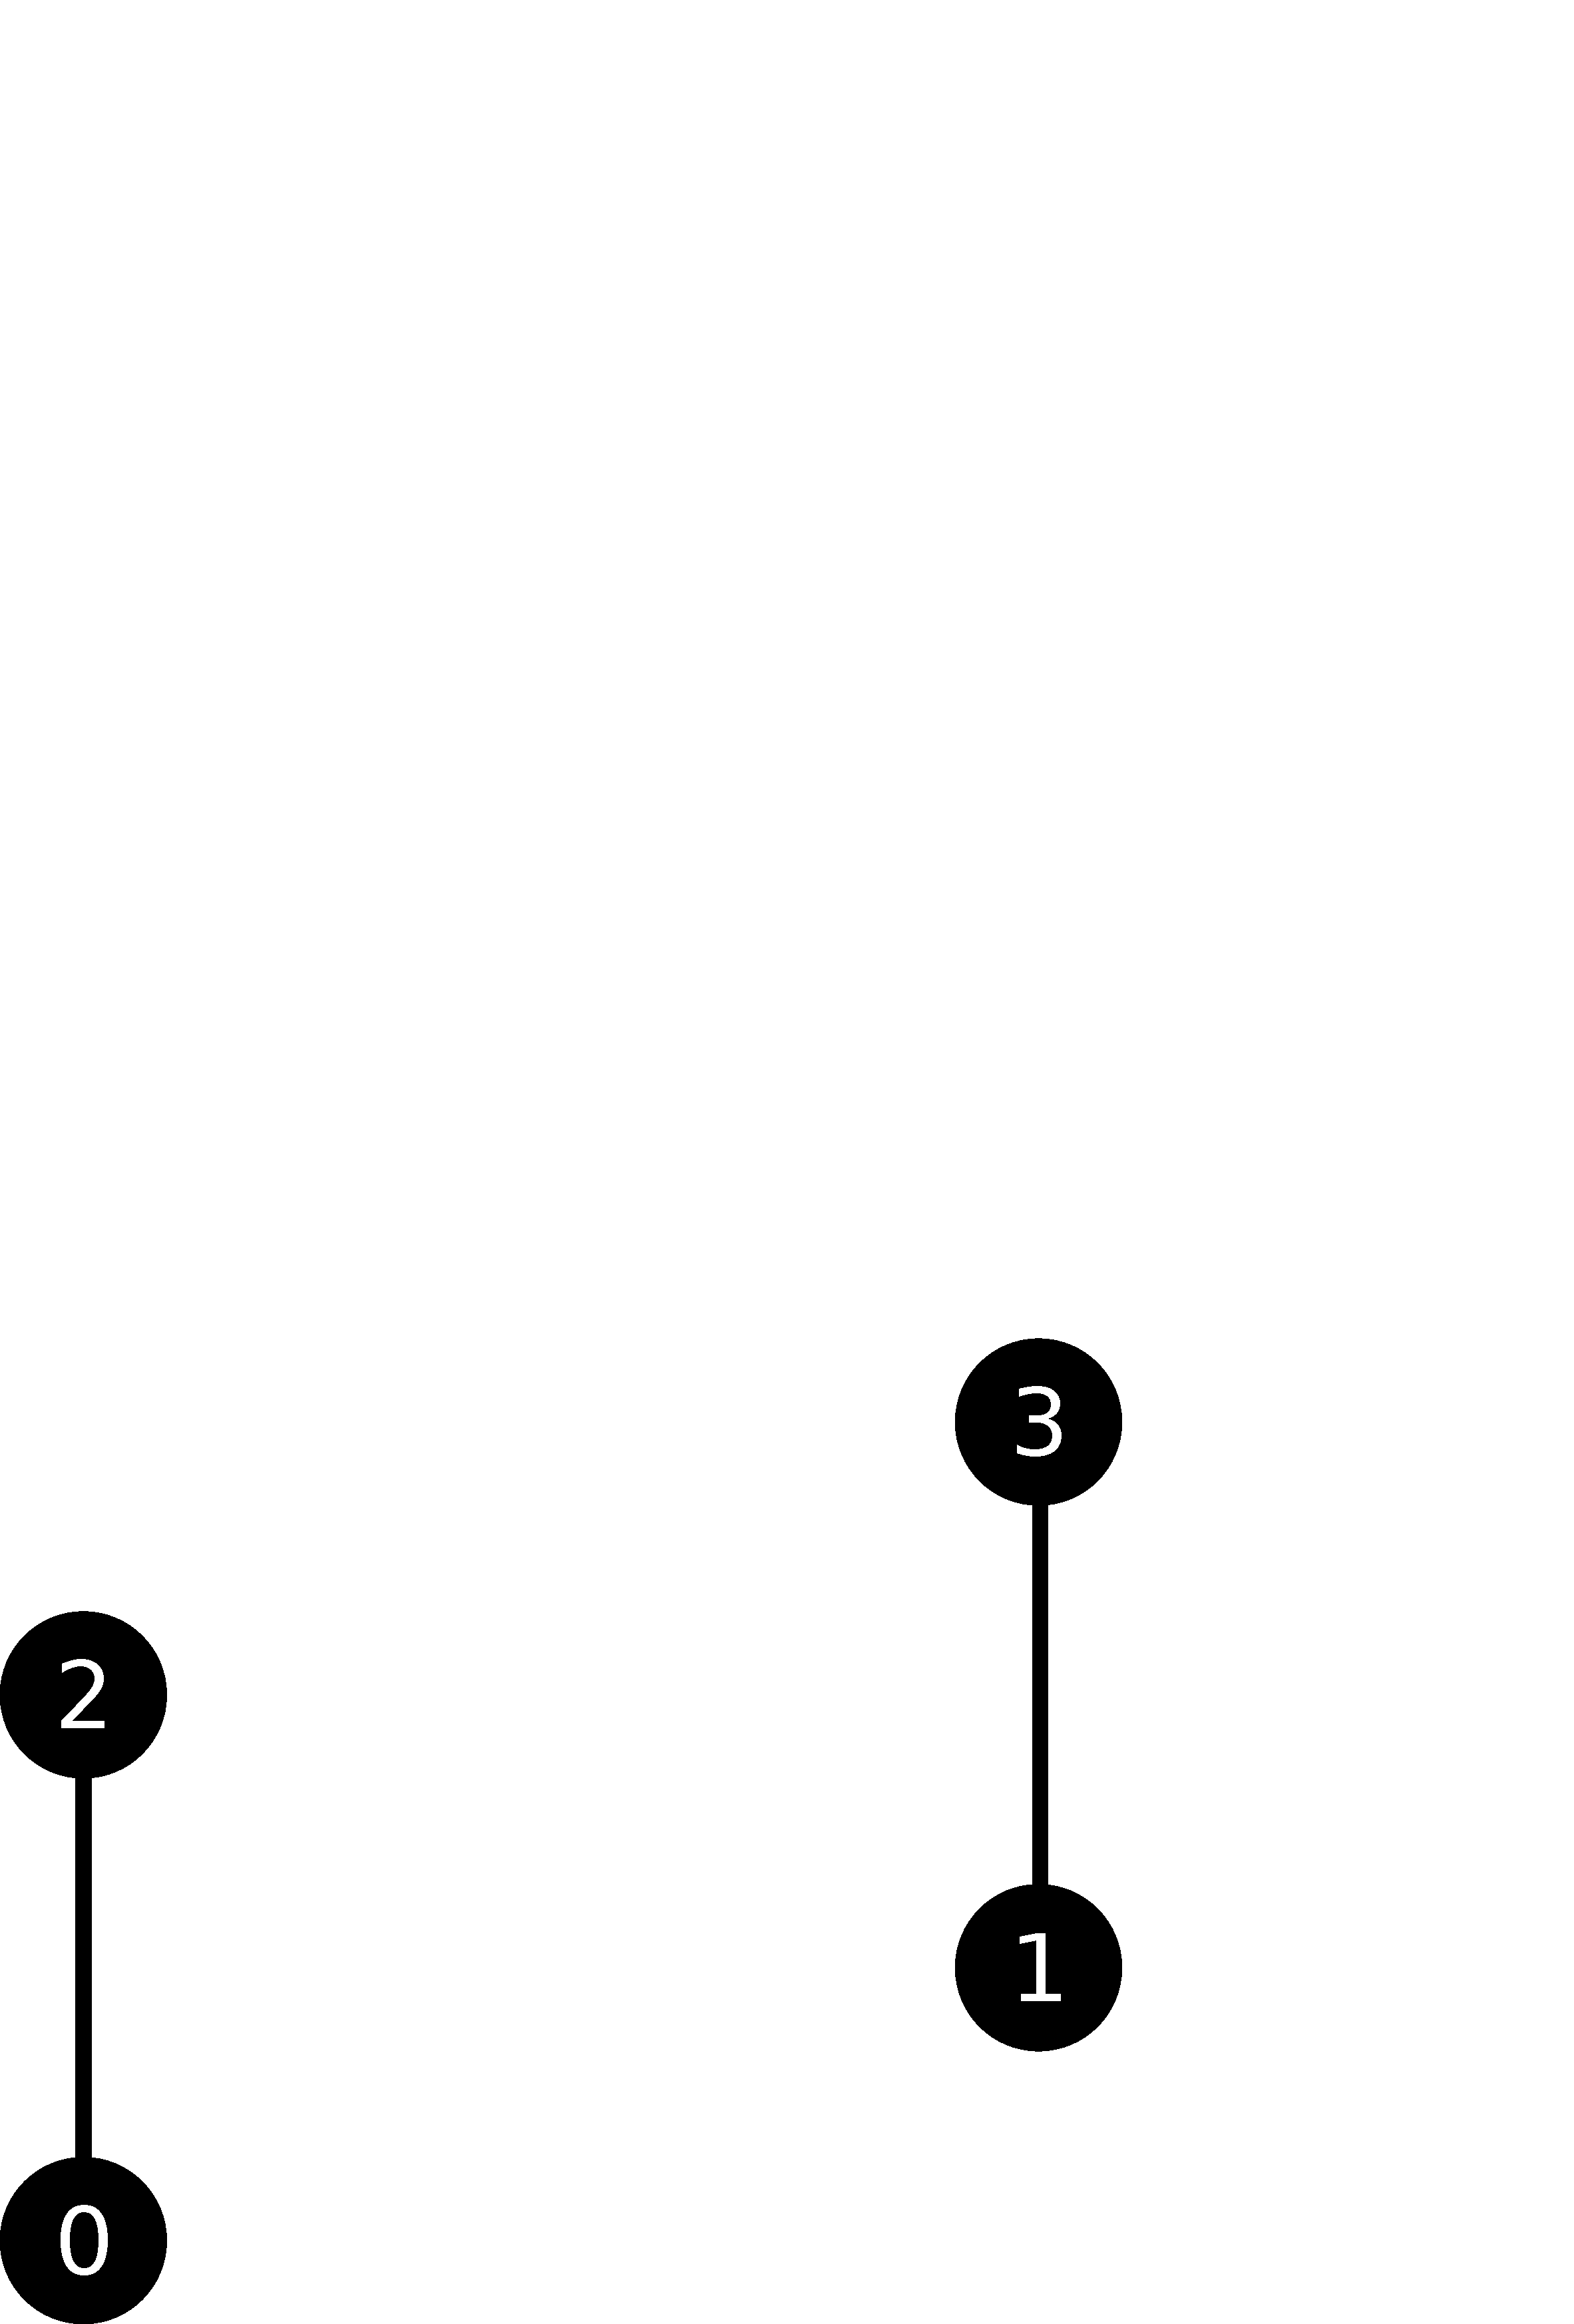
\includegraphics[scale=0.08]{./images/filtration/asc-tree/x4.pdf}}}%
    \qquad
    \subfloat[$CT(X)_4$]{{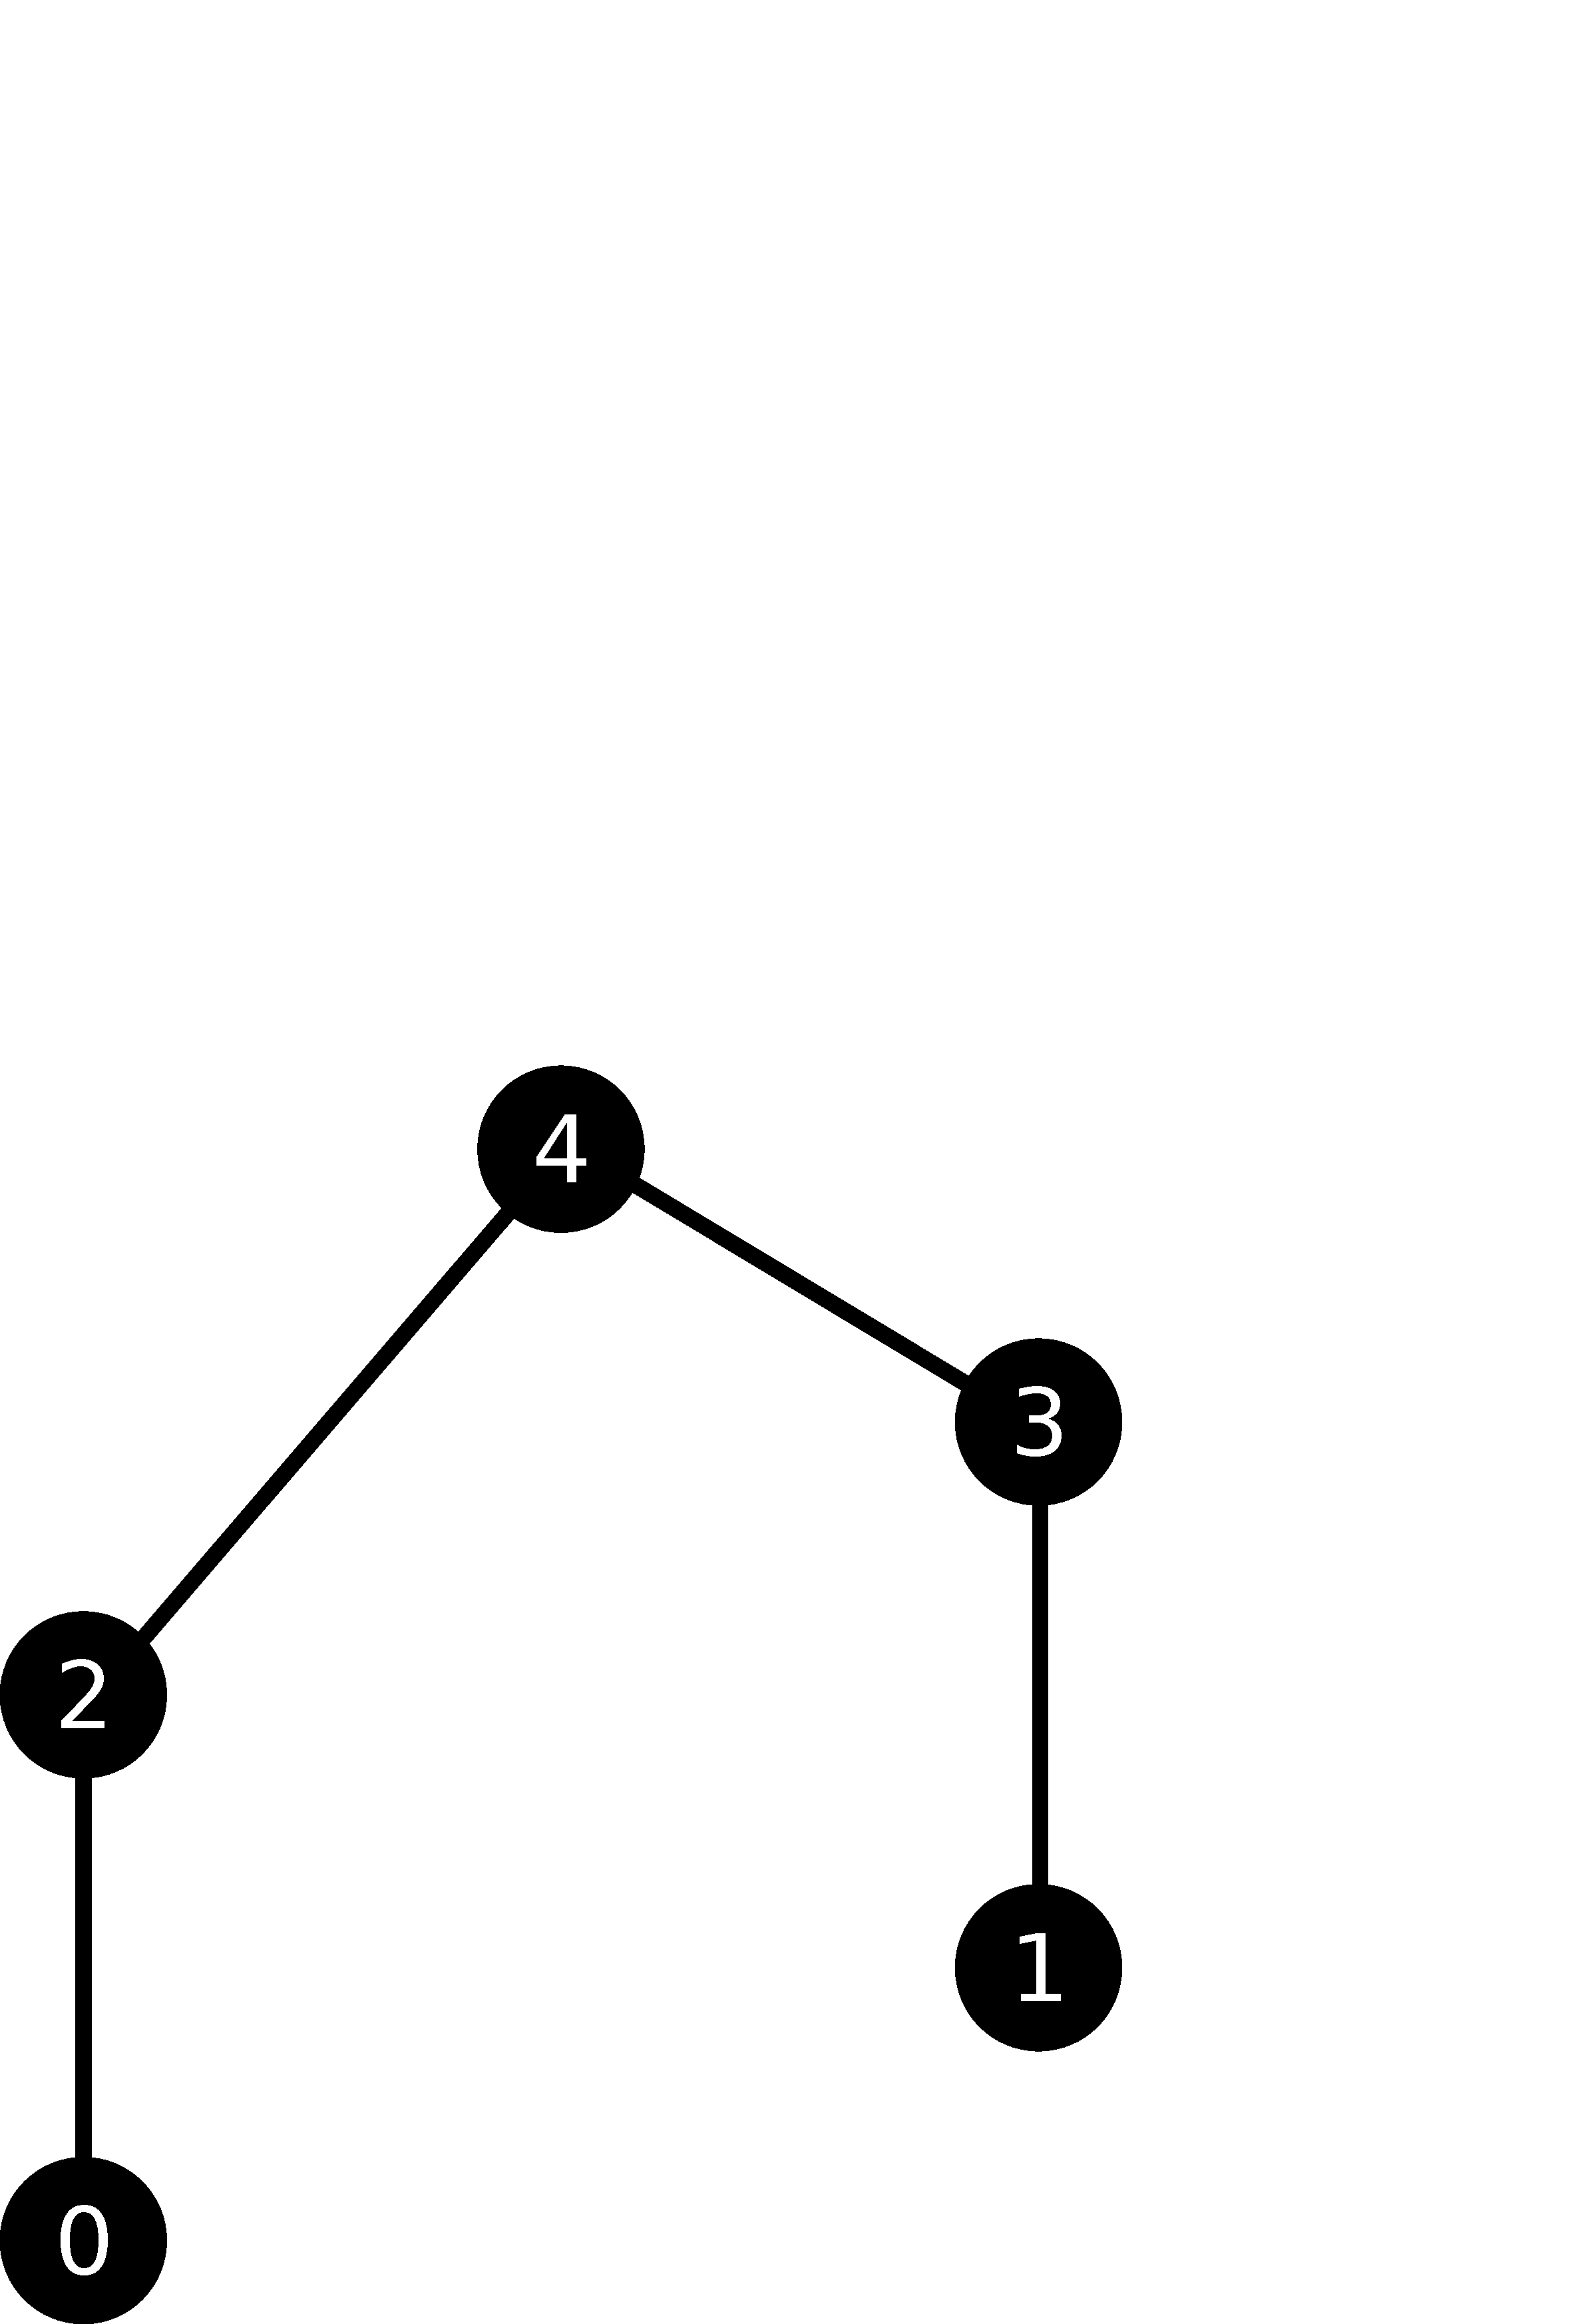
\includegraphics[scale=0.08]{./images/filtration/asc-tree/x5.pdf}}}%
    \qquad
    \subfloat[$CT(X)_5$]{{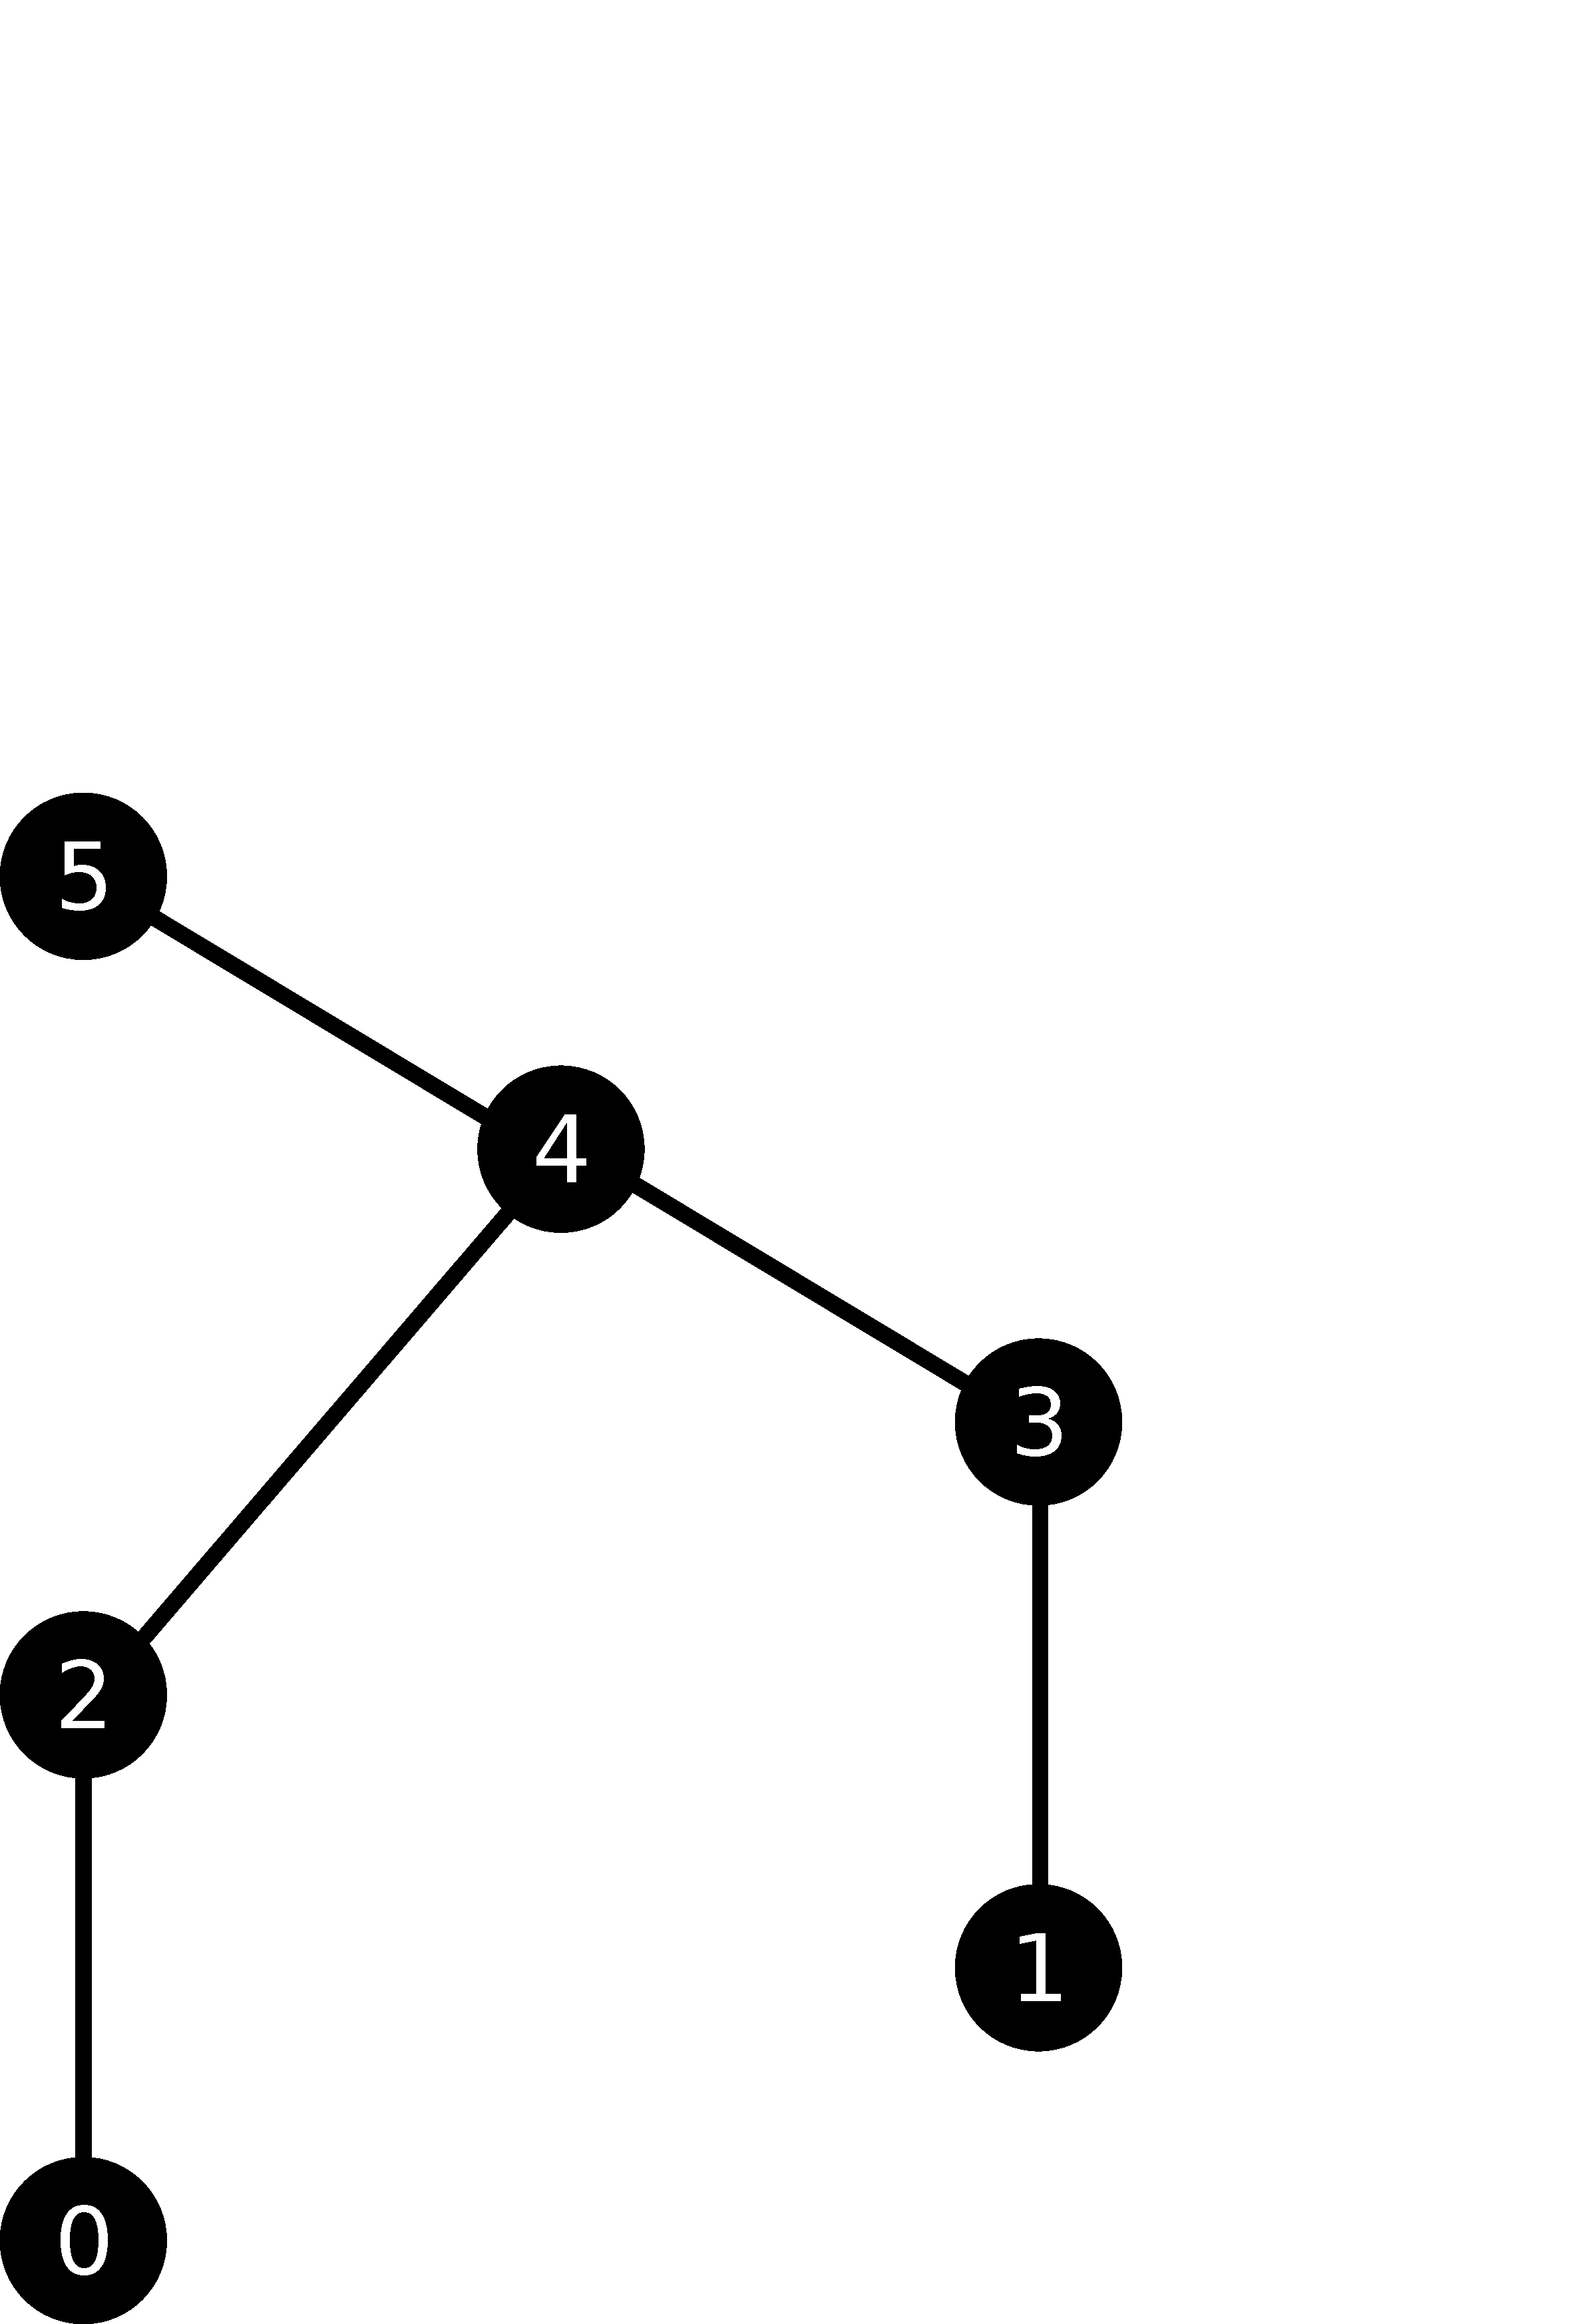
\includegraphics[scale=0.08]{./images/filtration/asc-tree/x6.pdf}}}%

    \par\bigskip

    \subfloat[$CT(X)_6$]{{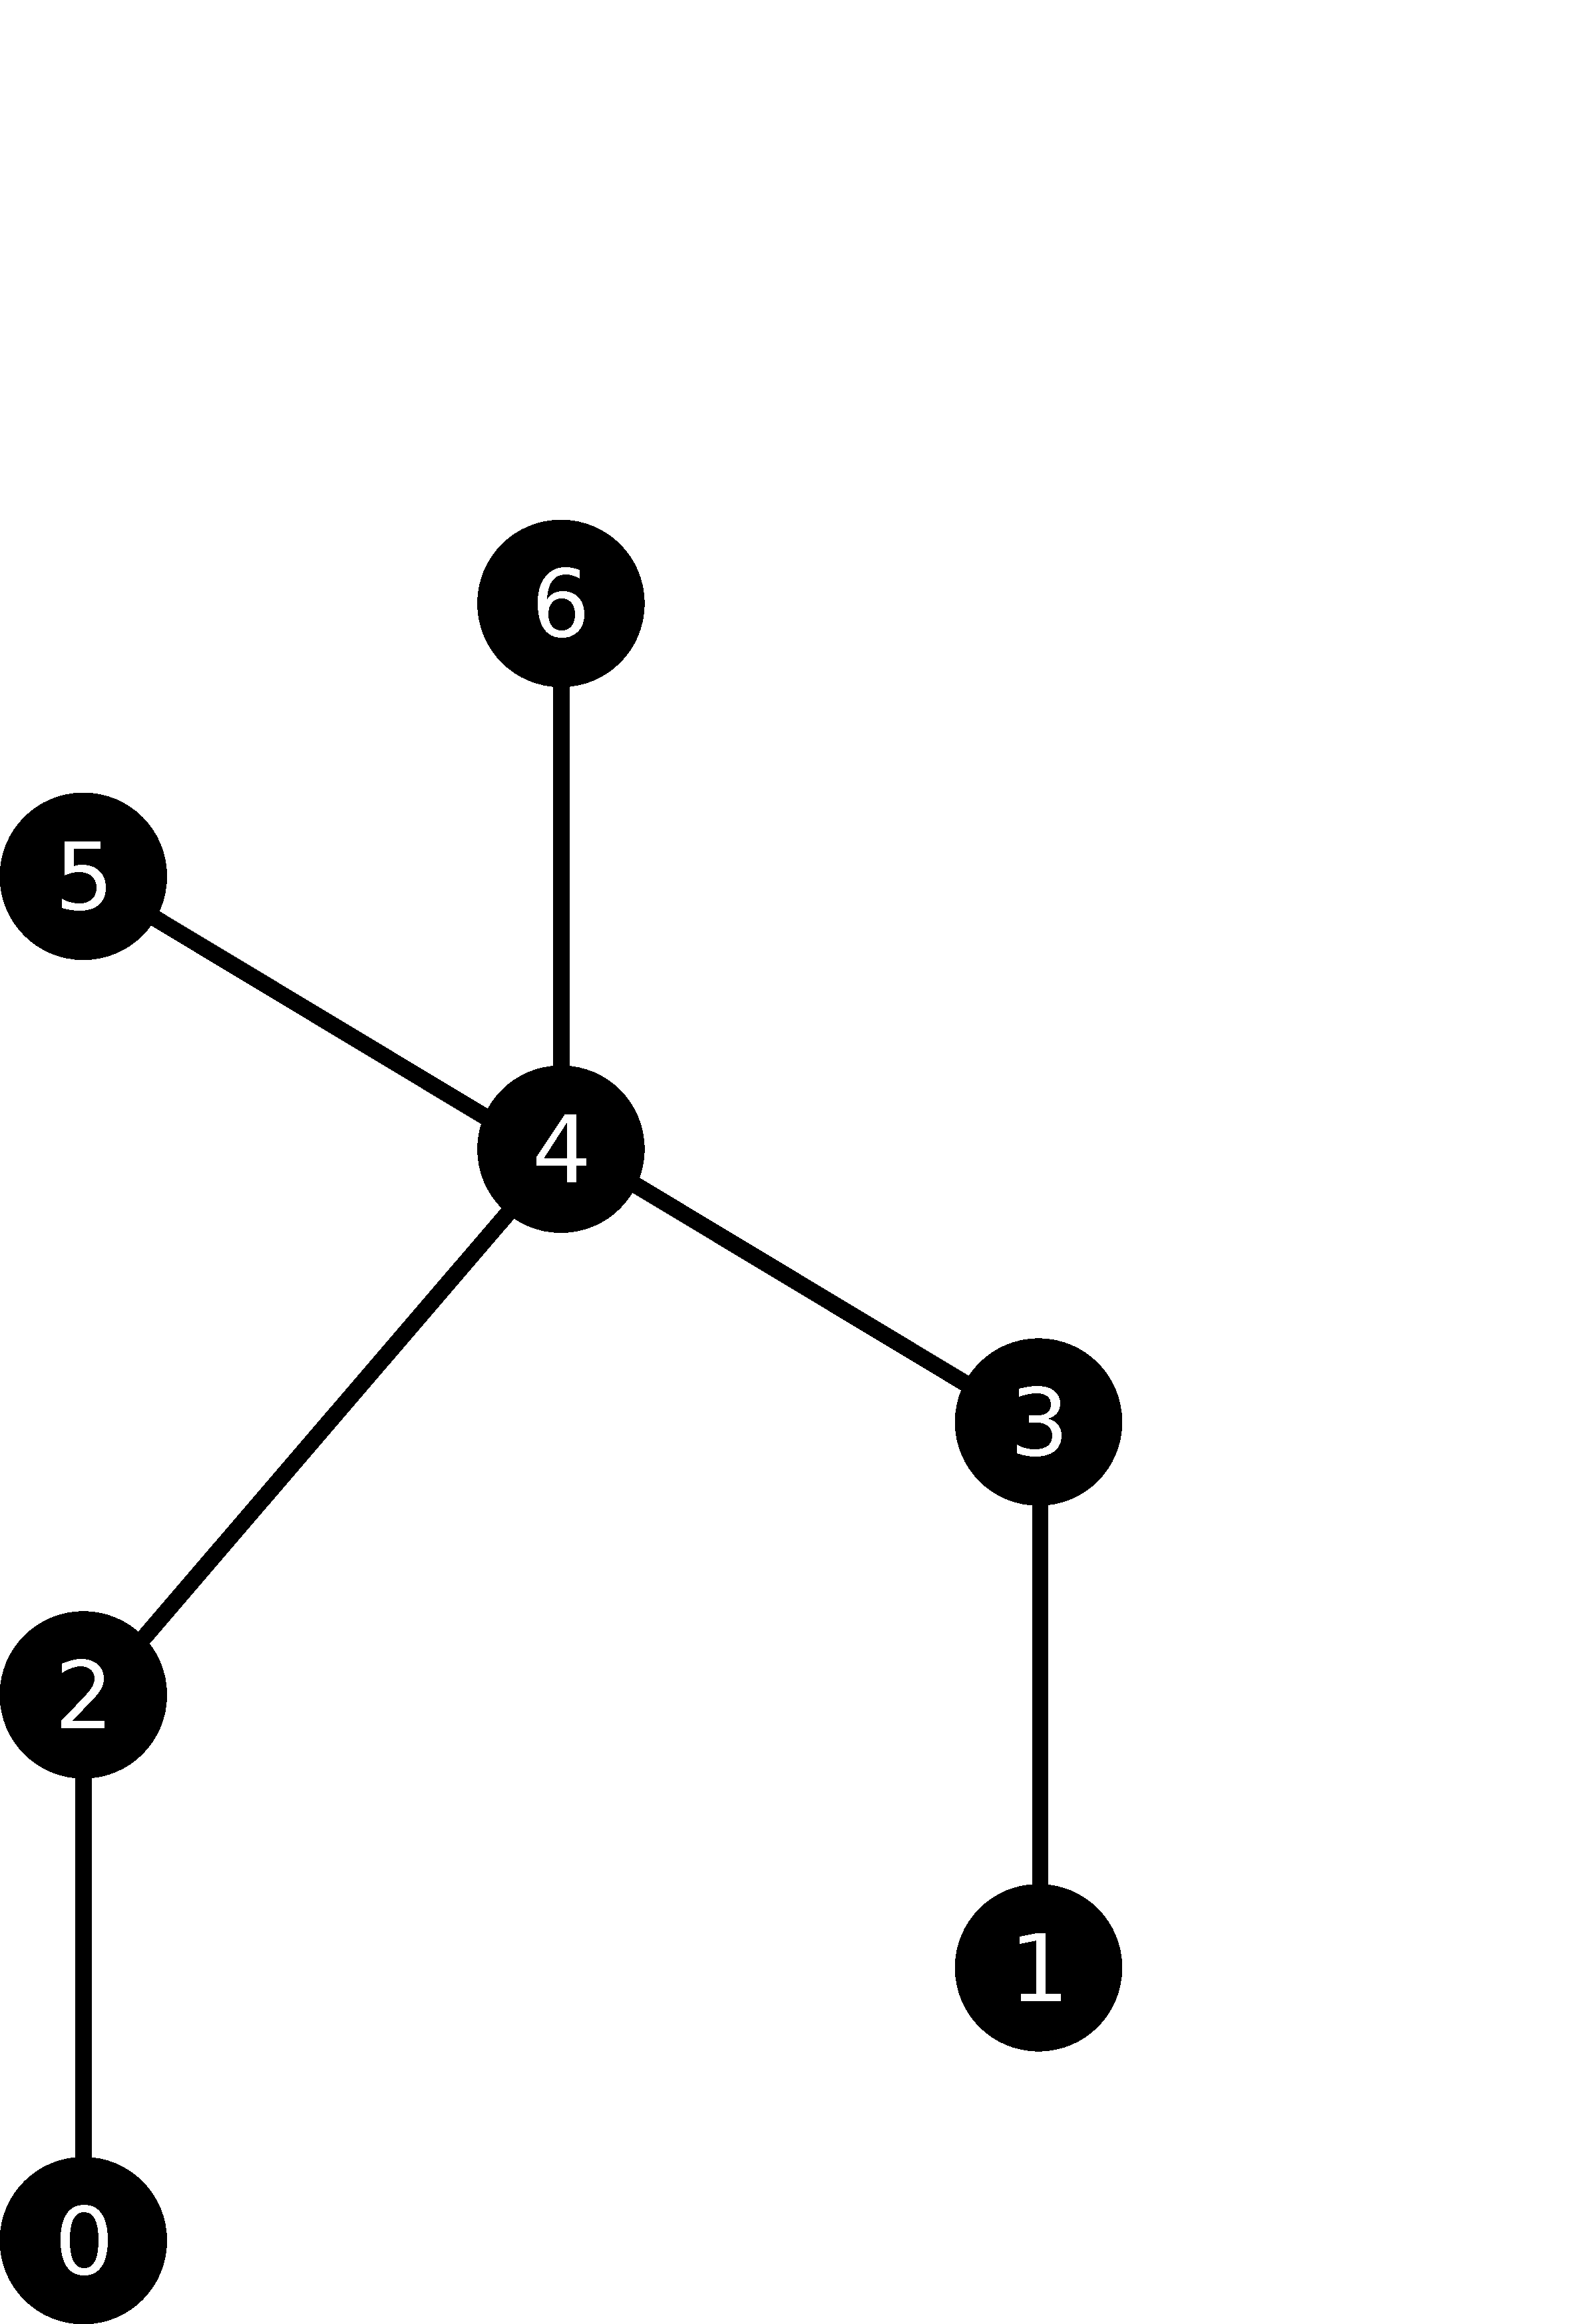
\includegraphics[scale=0.08]{./images/filtration/asc-tree/x7.pdf}}}%
    \qquad
    \subfloat[$CT(X)_7$]{{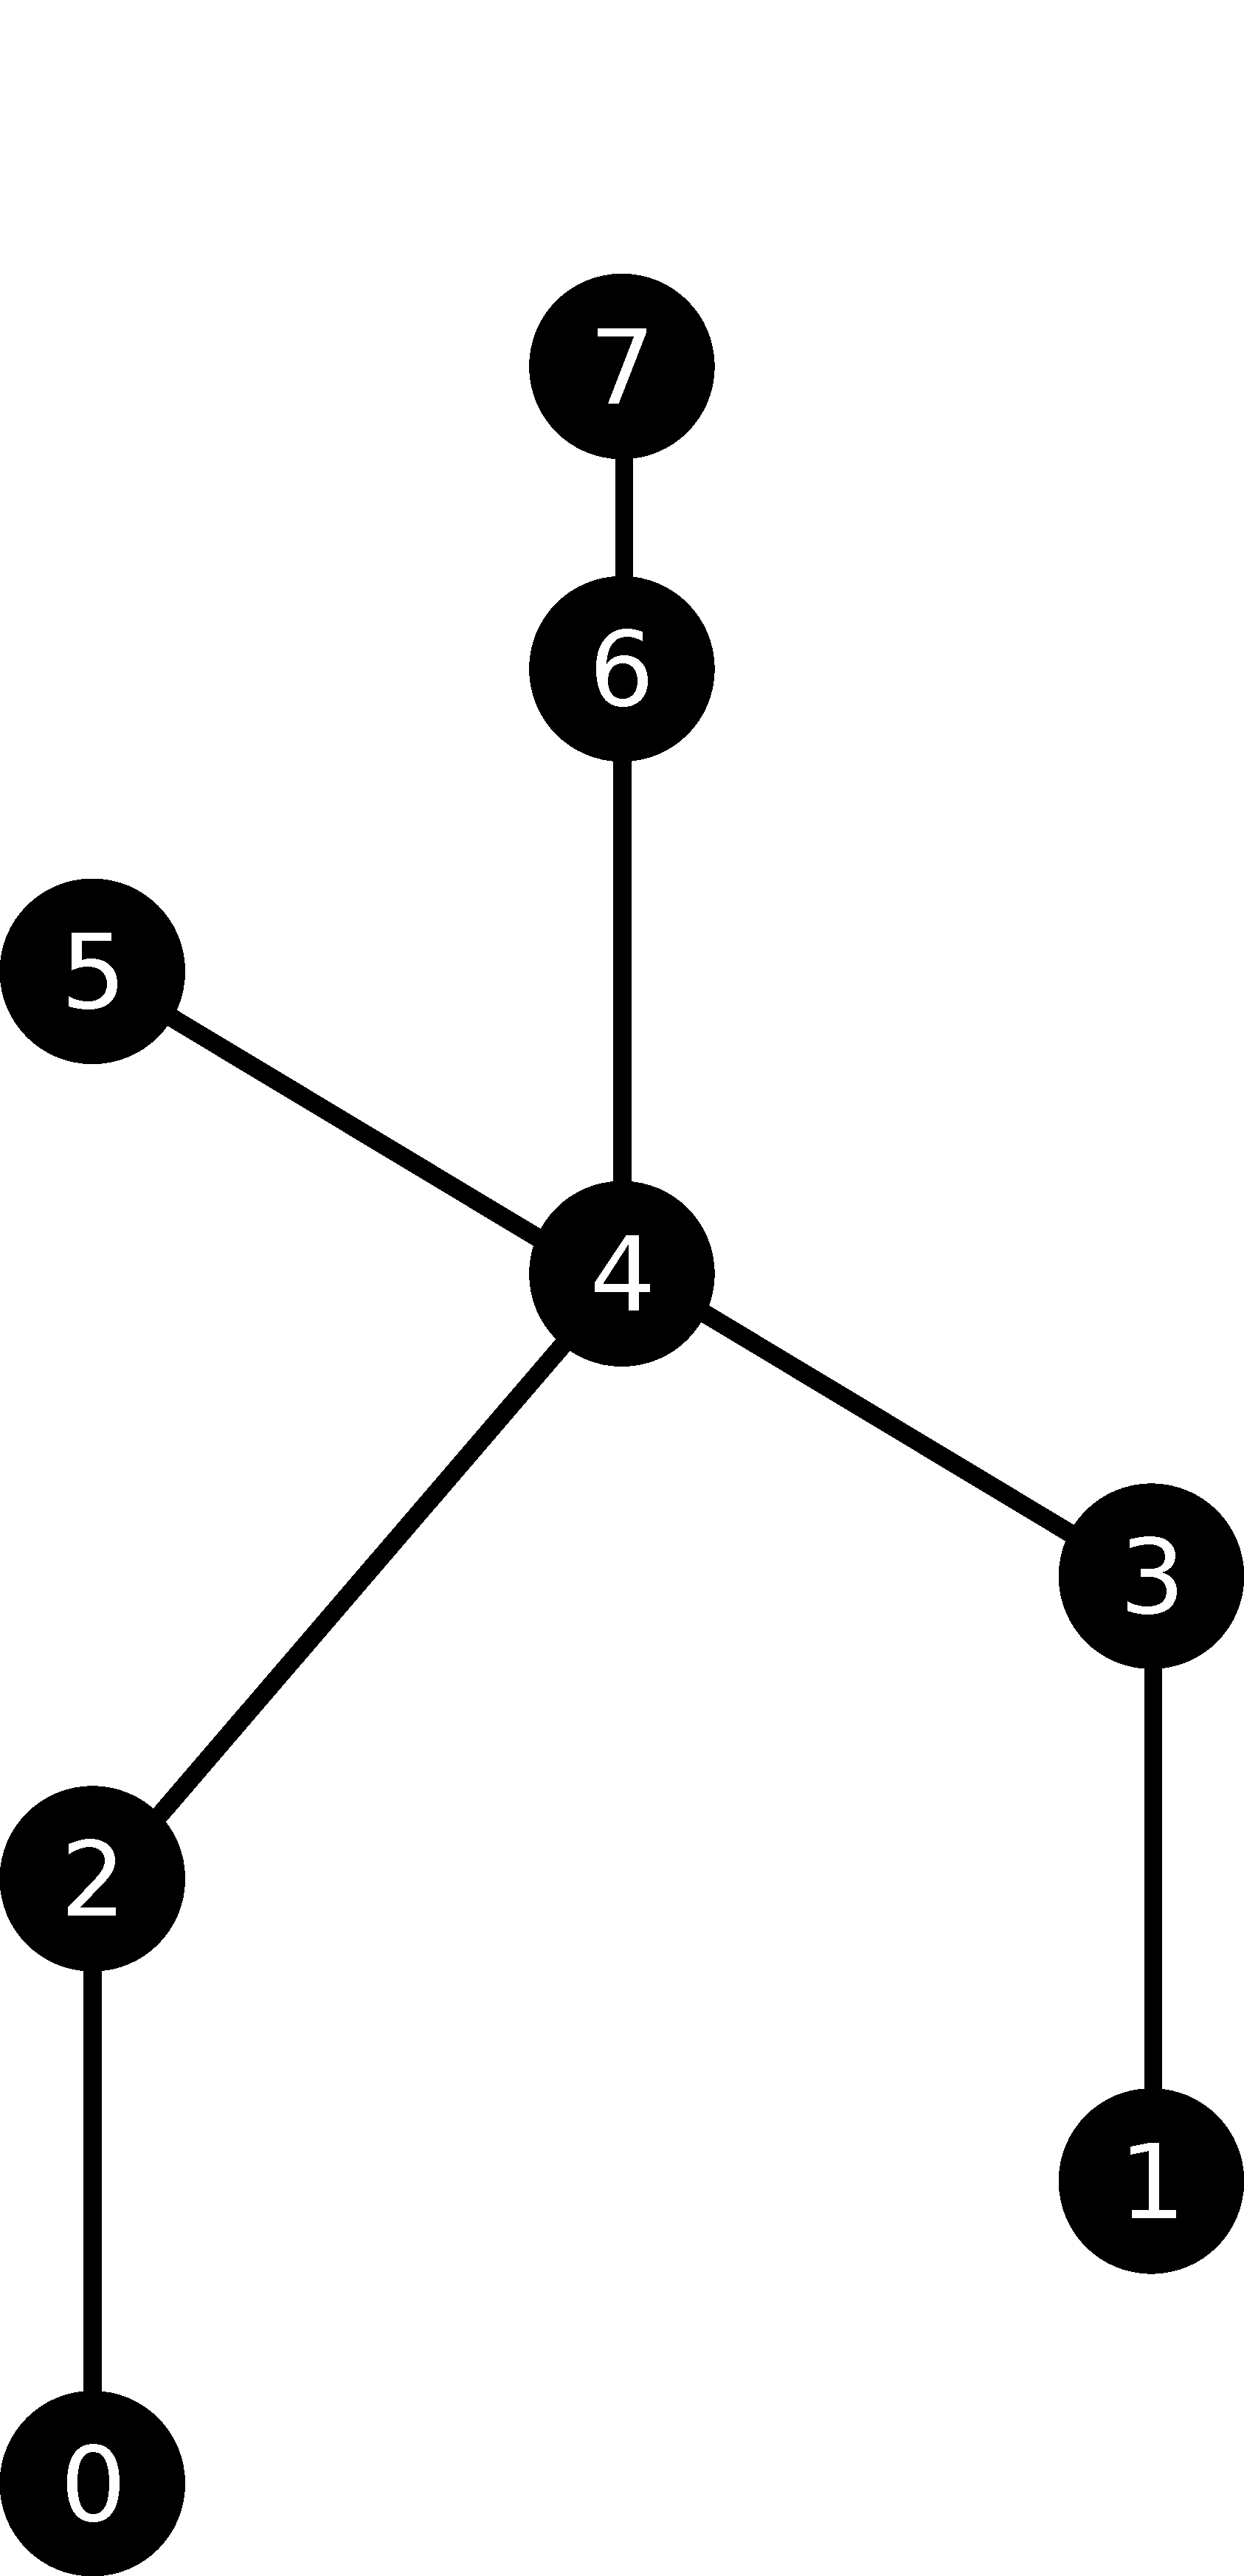
\includegraphics[scale=0.08]{./images/filtration/asc-tree/x8.pdf}}}%
    \qquad
    \subfloat[$CT(X)_8$]{{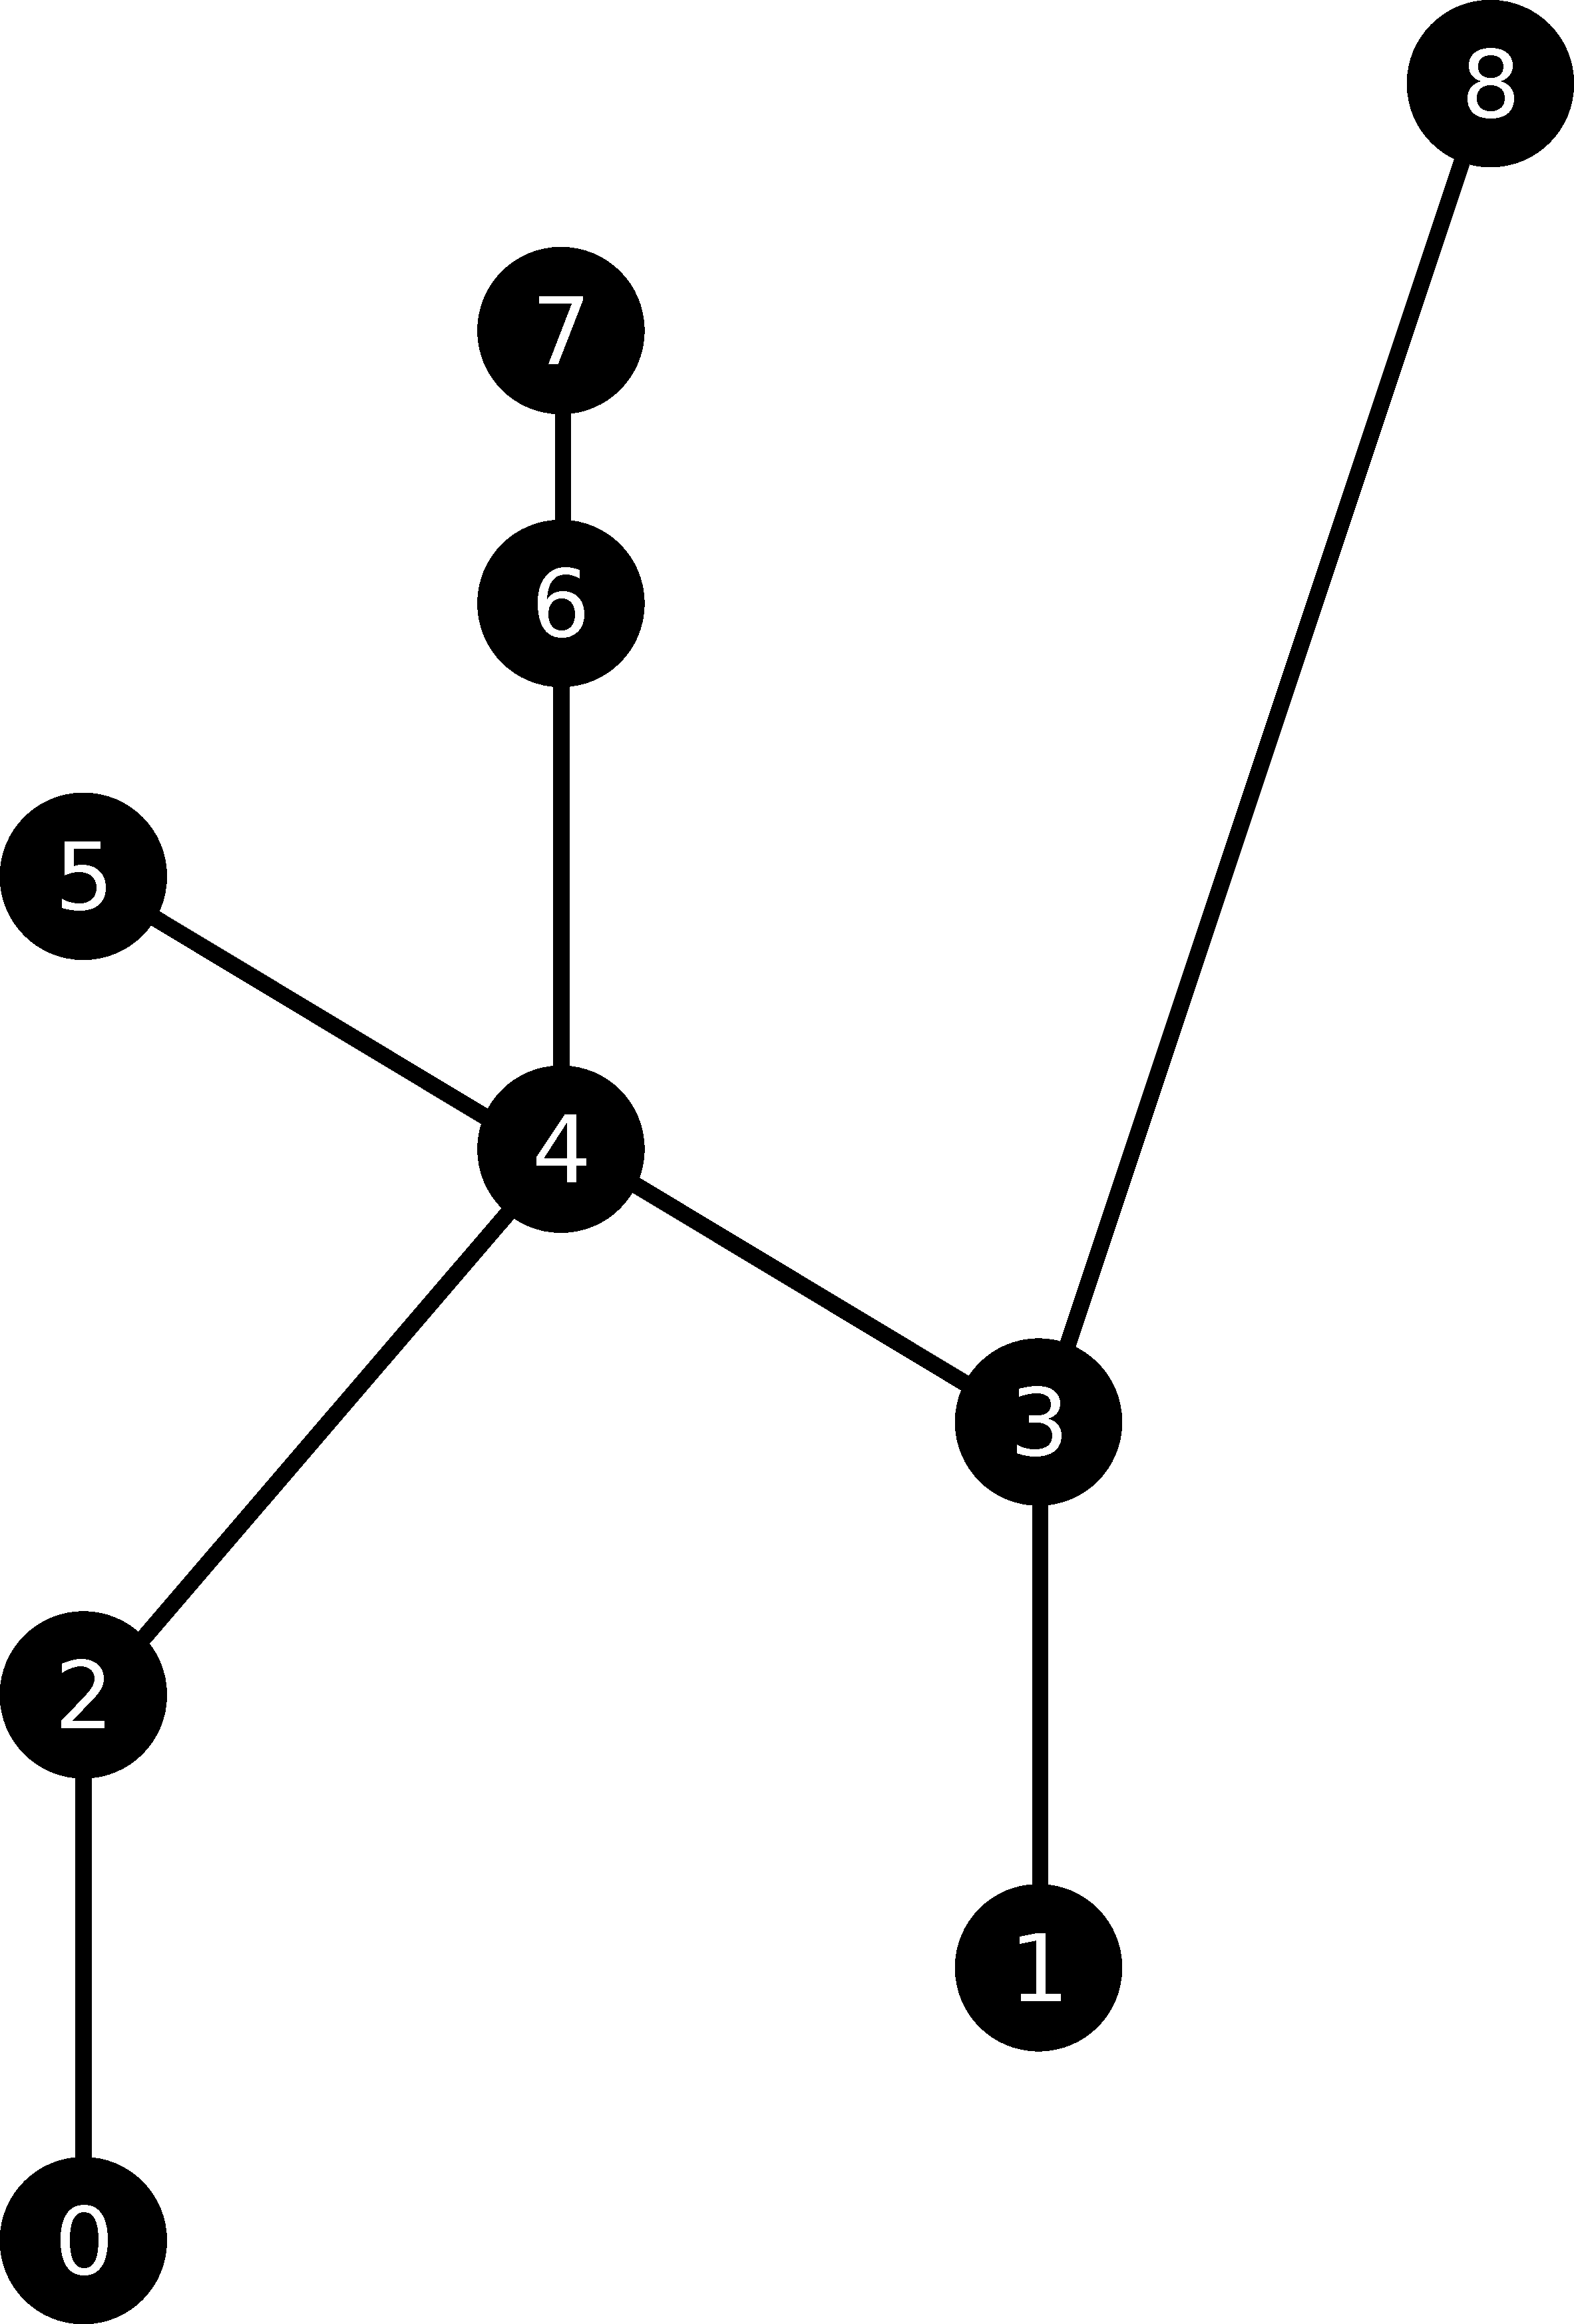
\includegraphics[scale=0.08]{./images/filtration/asc-tree/x9.pdf}}}%

    \caption{Ascending filtration of the contour tree from Figure \ref{fig:mesh-join-split-contour} b.}%
    \label{fig:asc-filtration-tree}%
\end{figure}


\chapter{Descending Filtration of the Contour Tree}
\label{chapter-desc}

\begin{figure}[h]%
    \captionsetup[subfigure]{labelformat=empty}
    \centering
    \subfloat[$CT(X)^9$]{{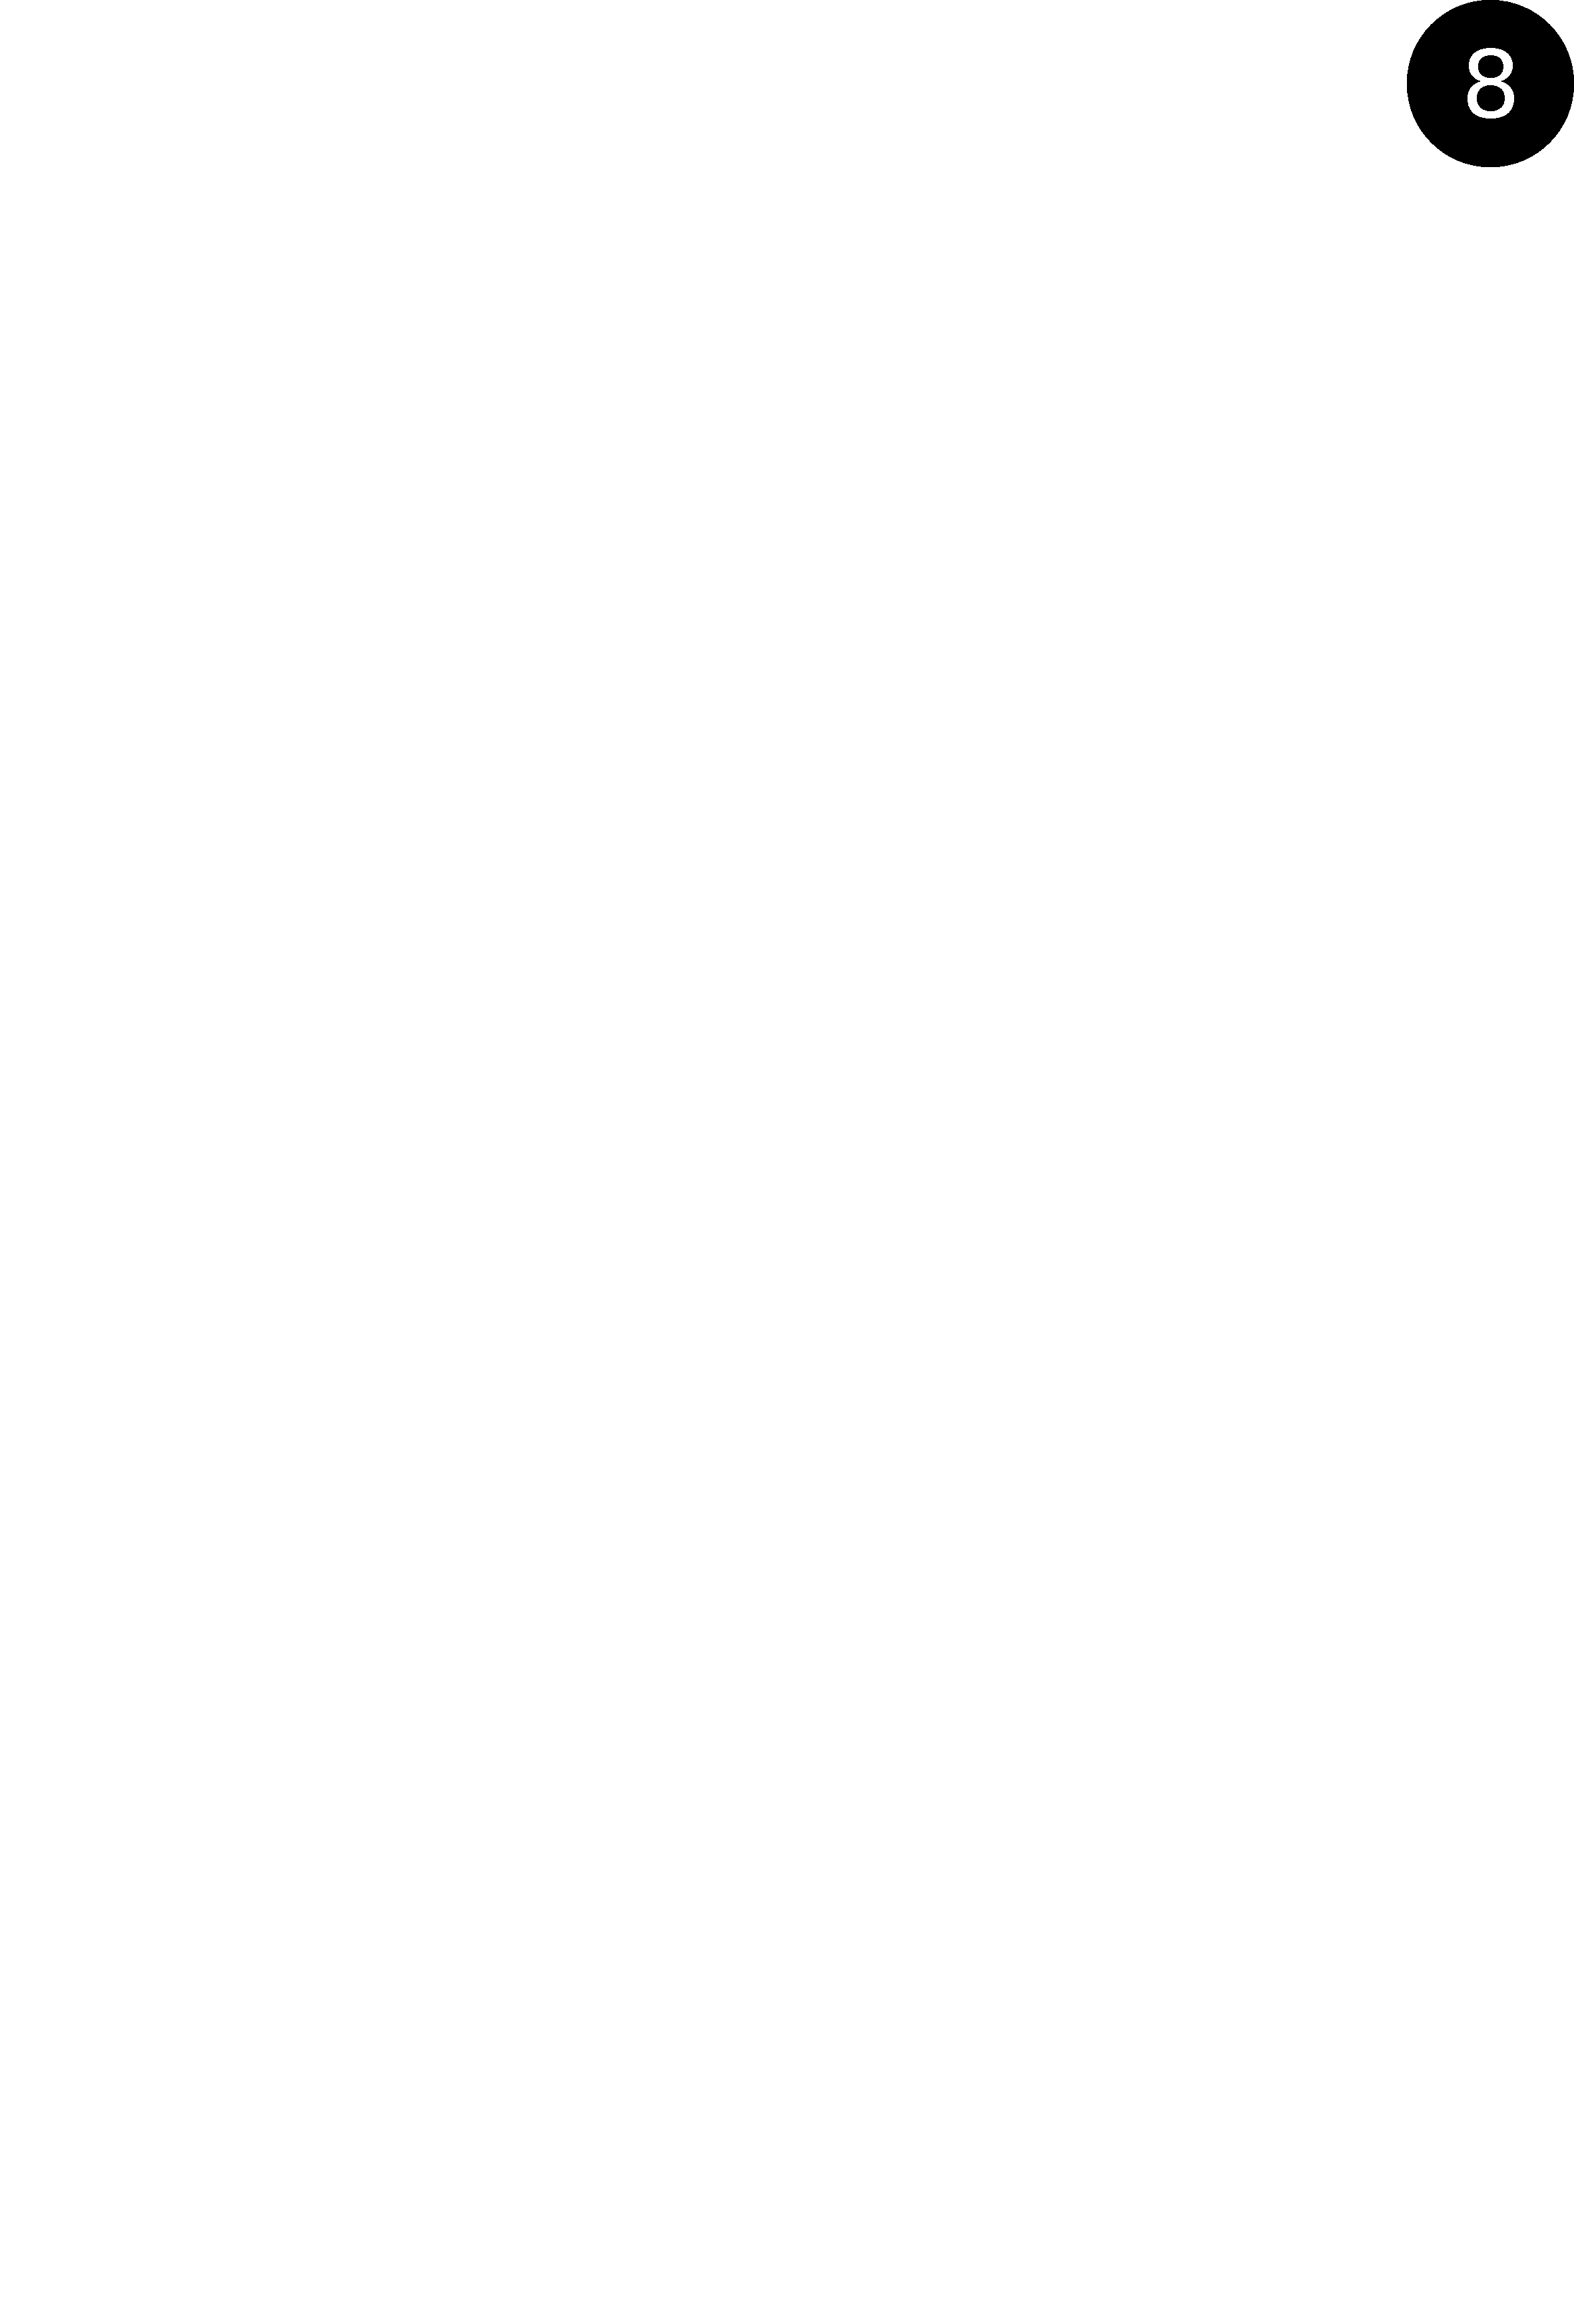
\includegraphics[scale=0.08]{./images/filtration/desc-tree/x1.pdf}}}%
    \qquad \qquad
    \subfloat[$CT(X)^8$]{{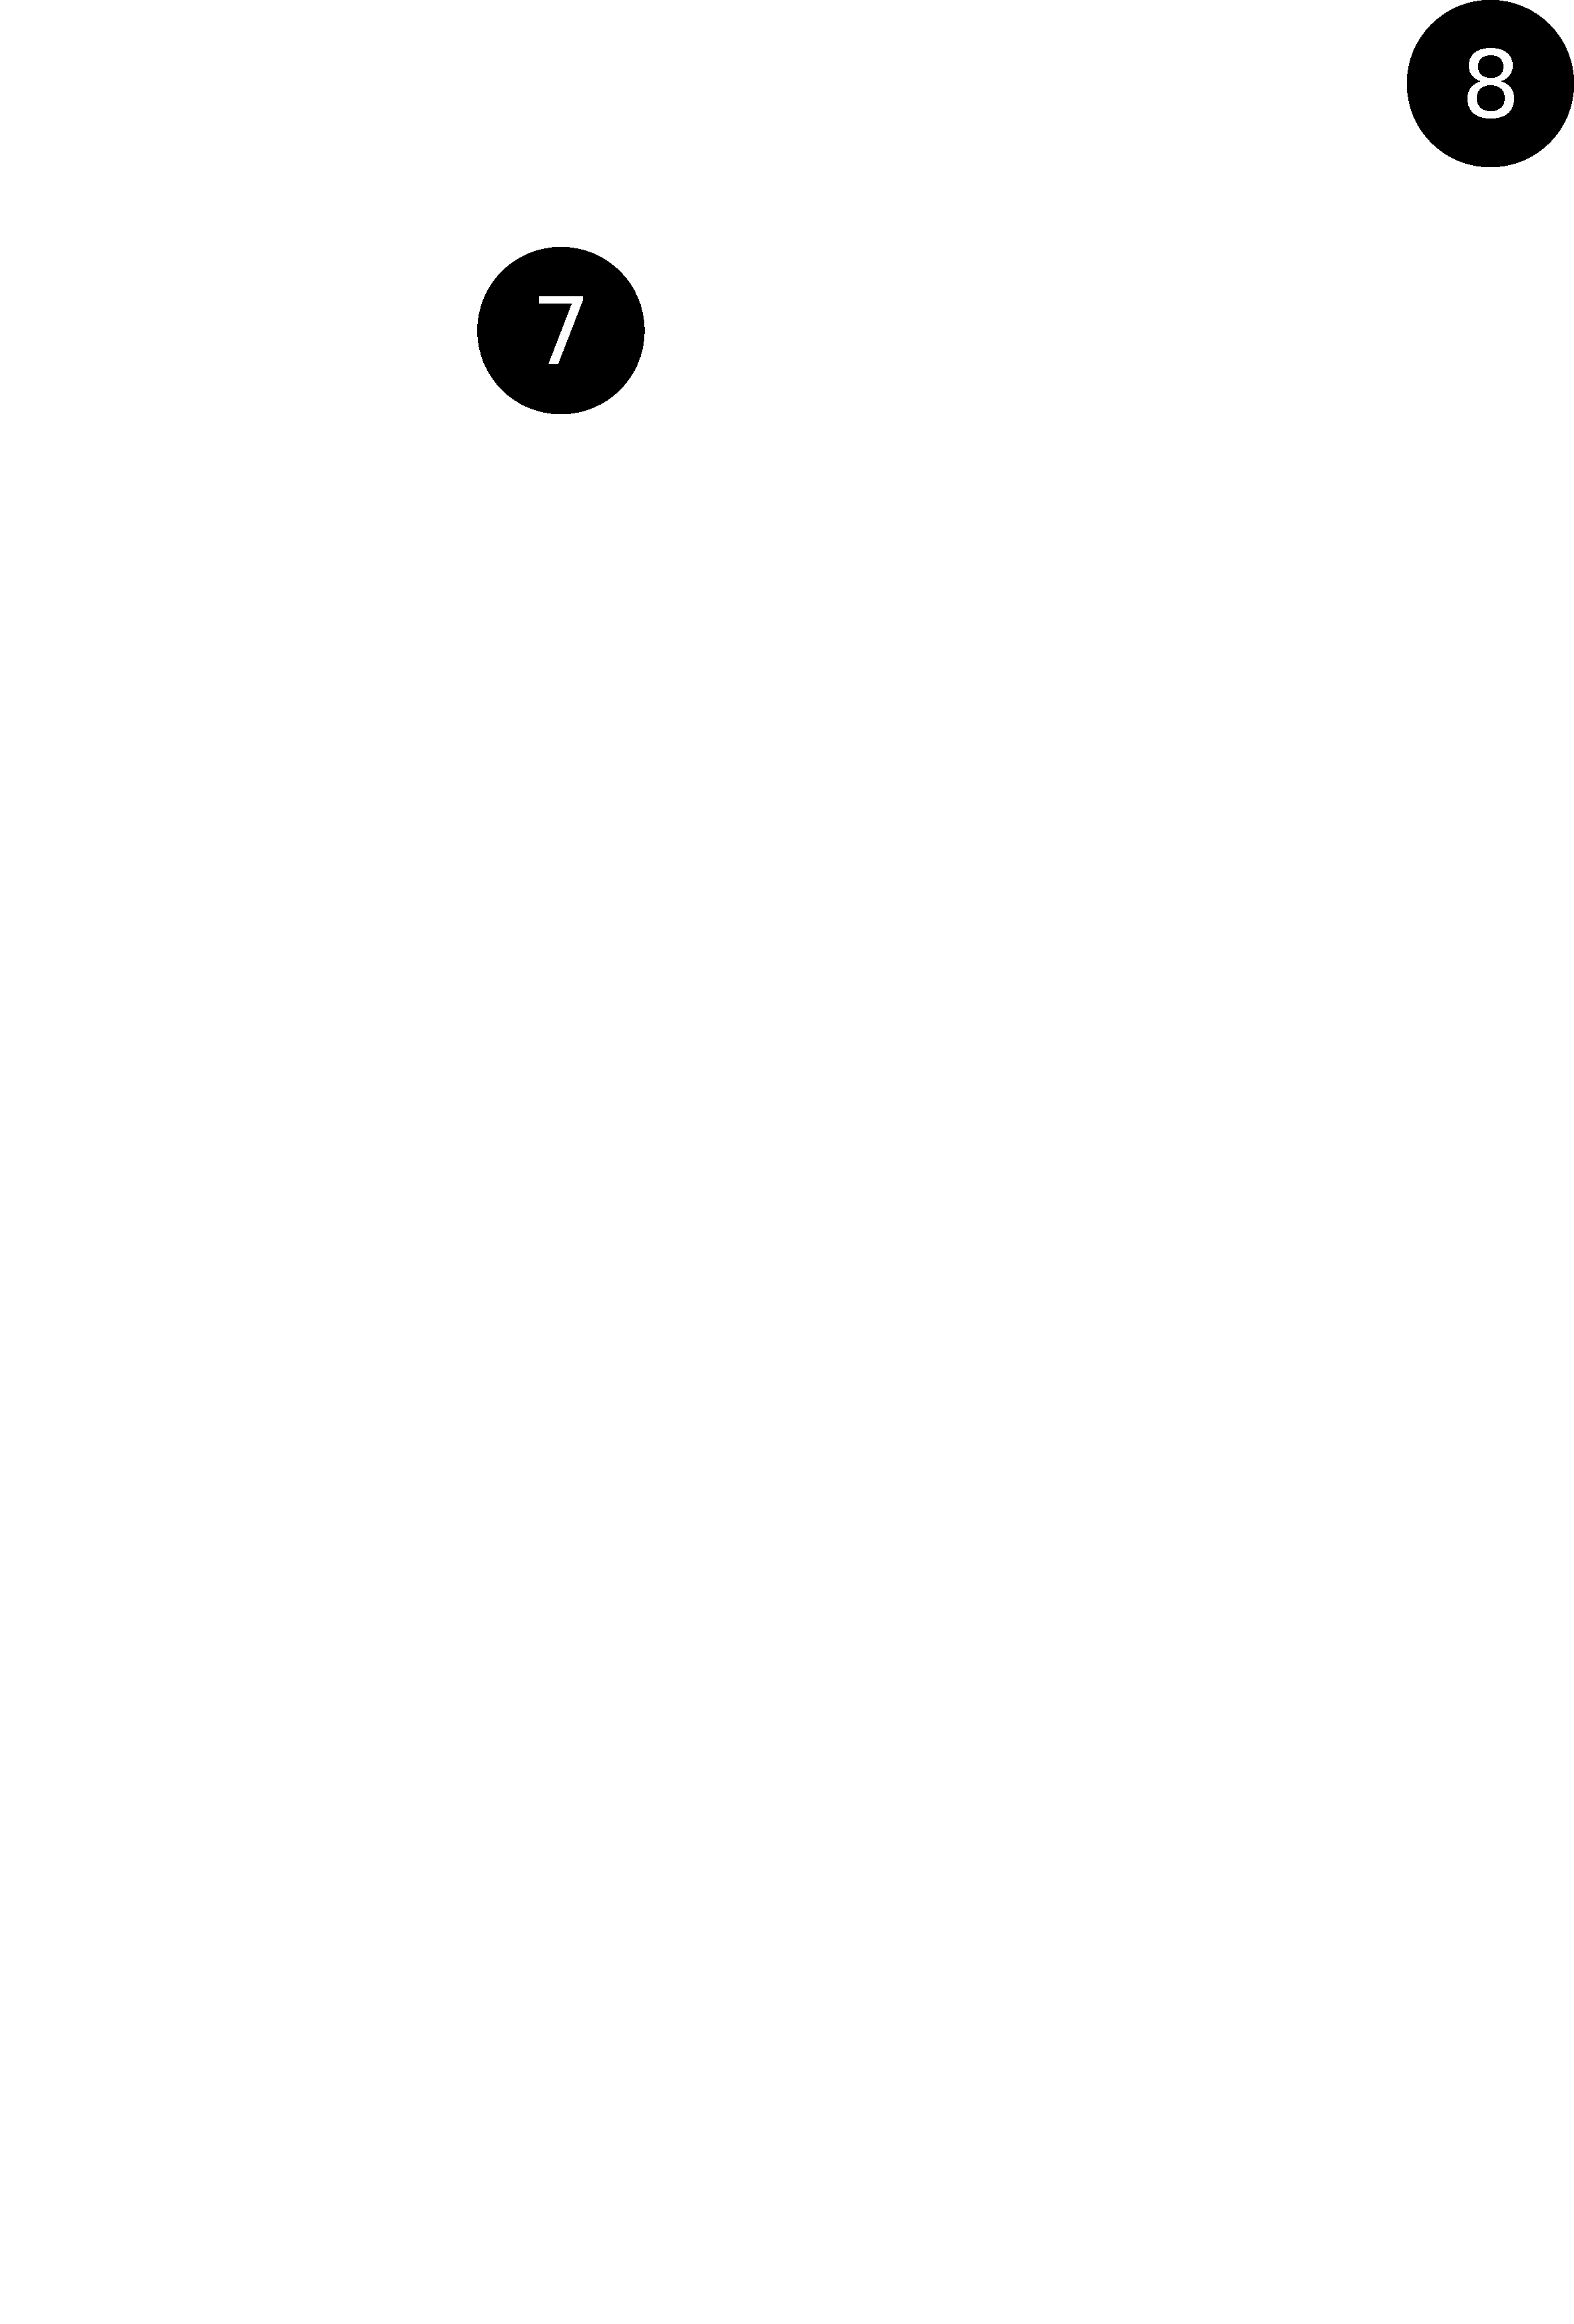
\includegraphics[scale=0.08]{./images/filtration/desc-tree/x2.pdf}}}%
    \qquad \qquad
    \subfloat[$CT(X)^7$]{{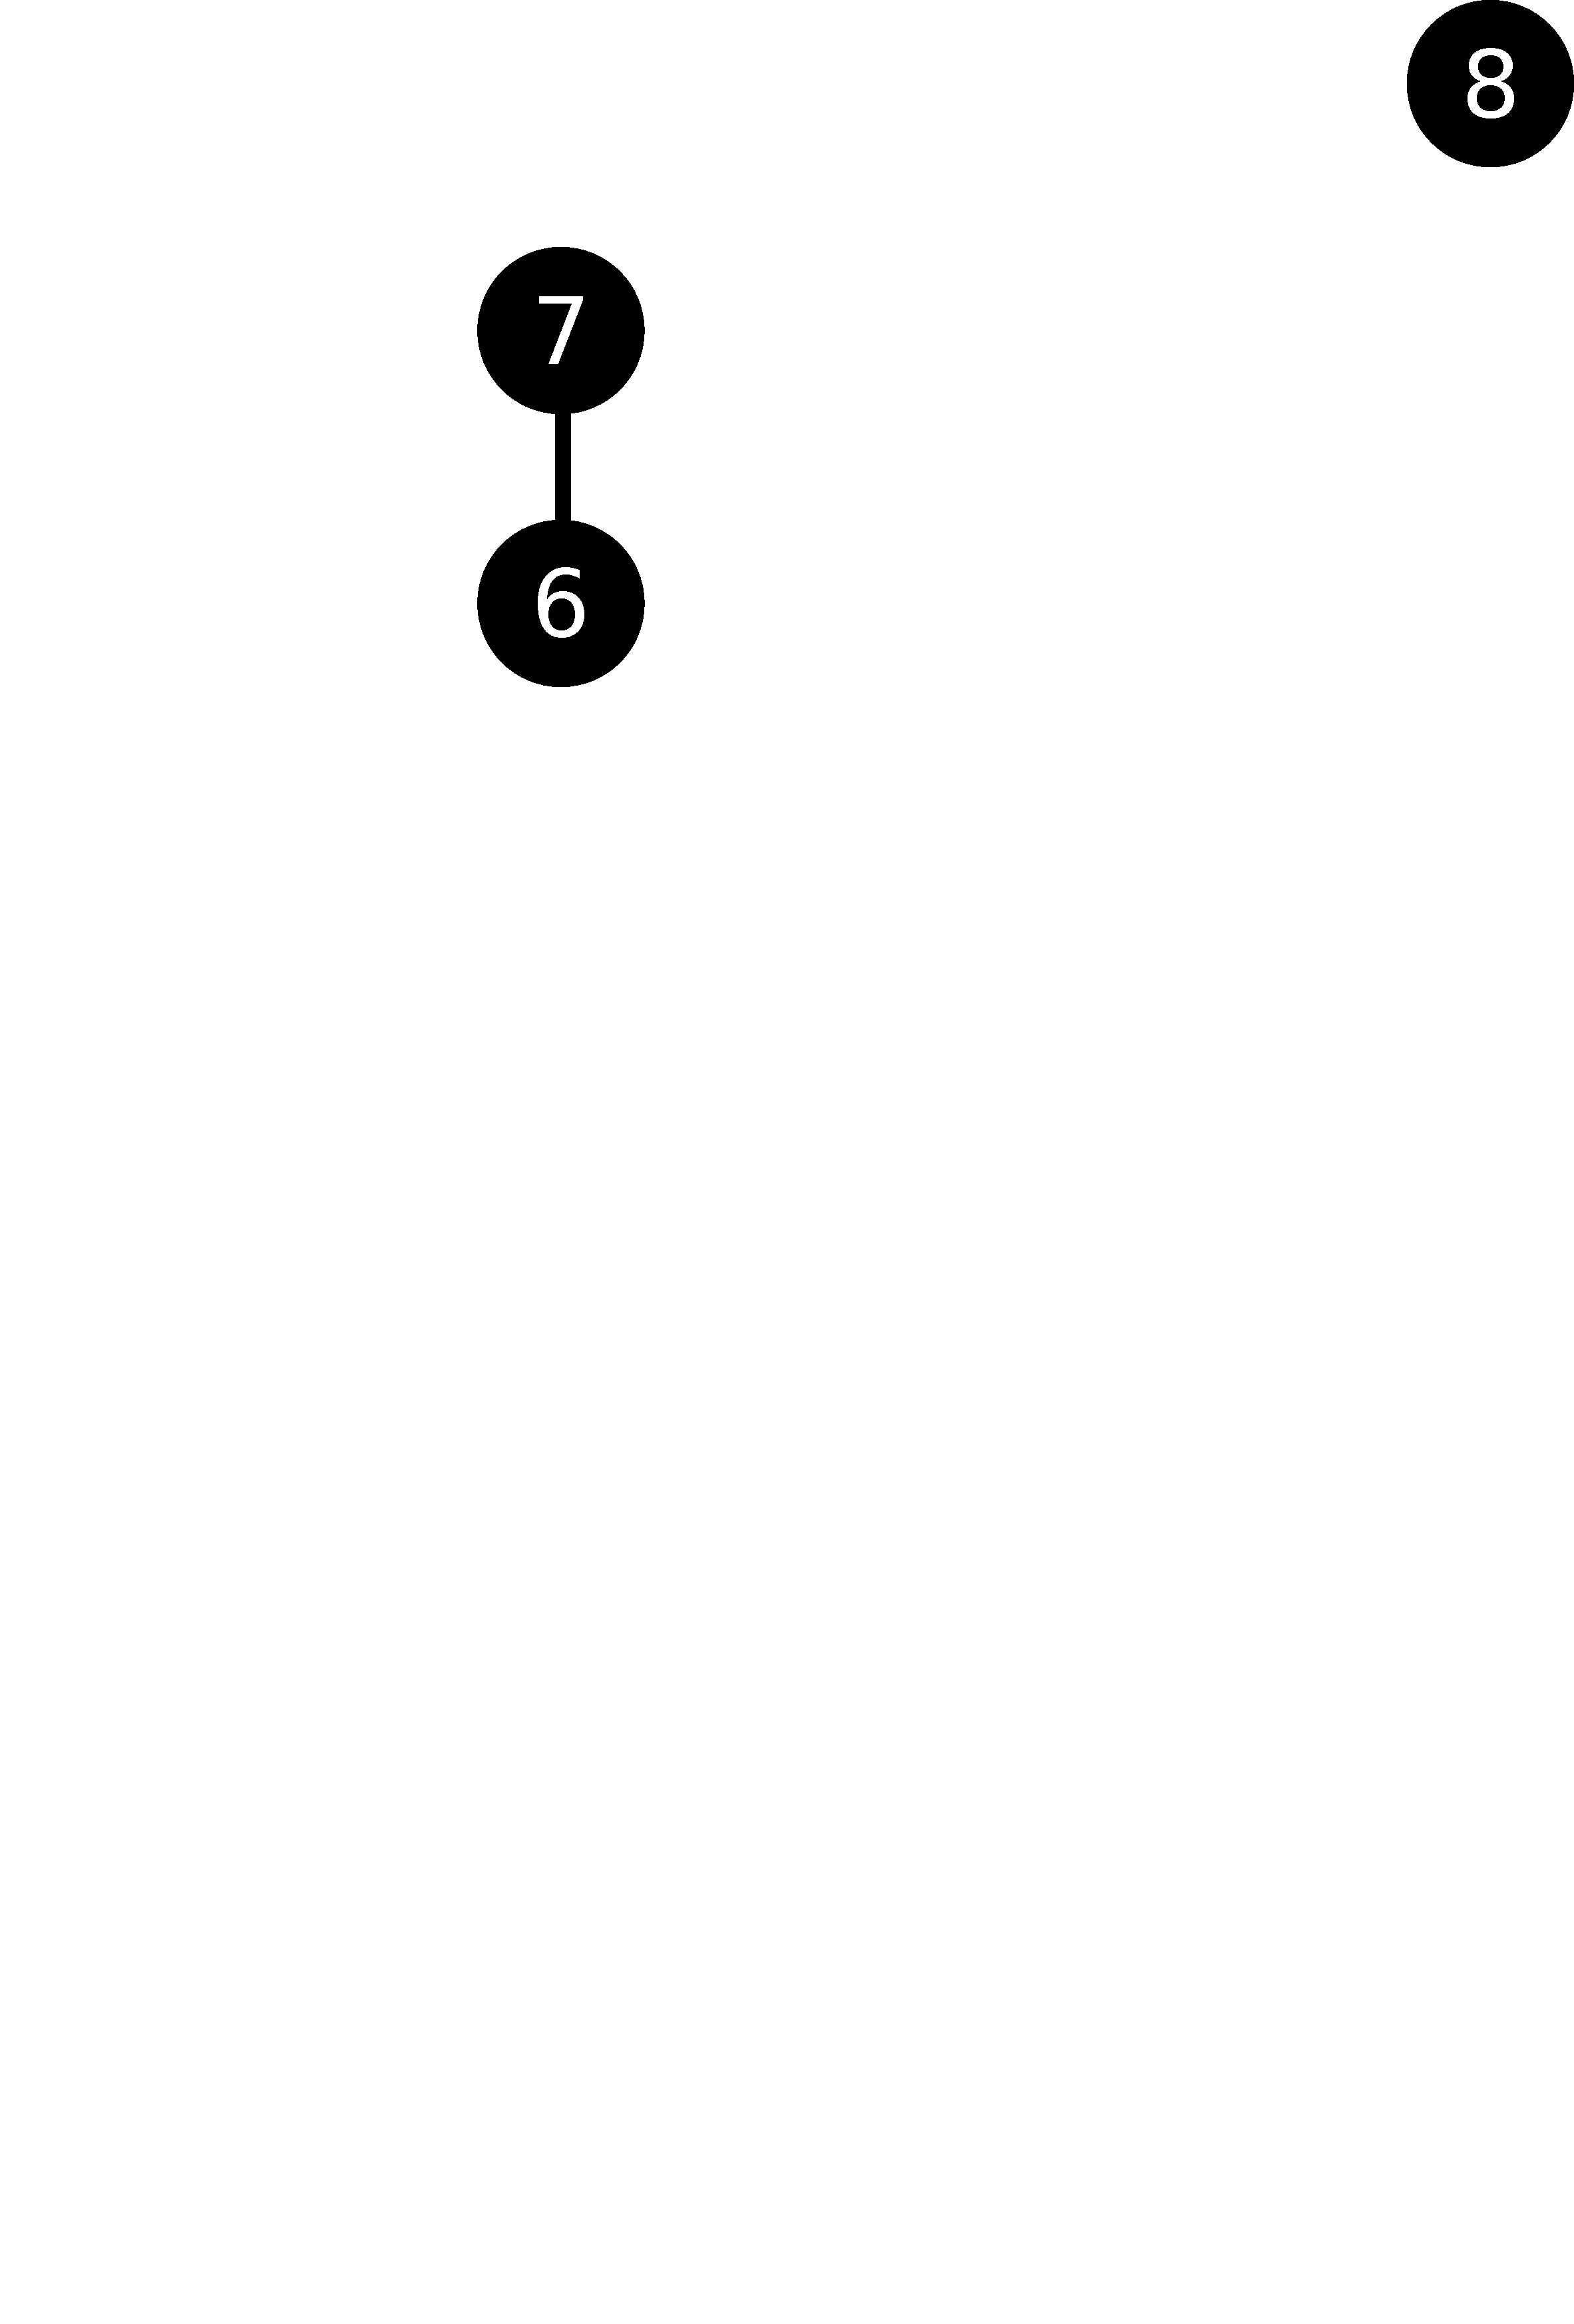
\includegraphics[scale=0.08]{./images/filtration/desc-tree/x3.pdf}}}%

    \par\bigskip

    \subfloat[$CT(X)^6$]{{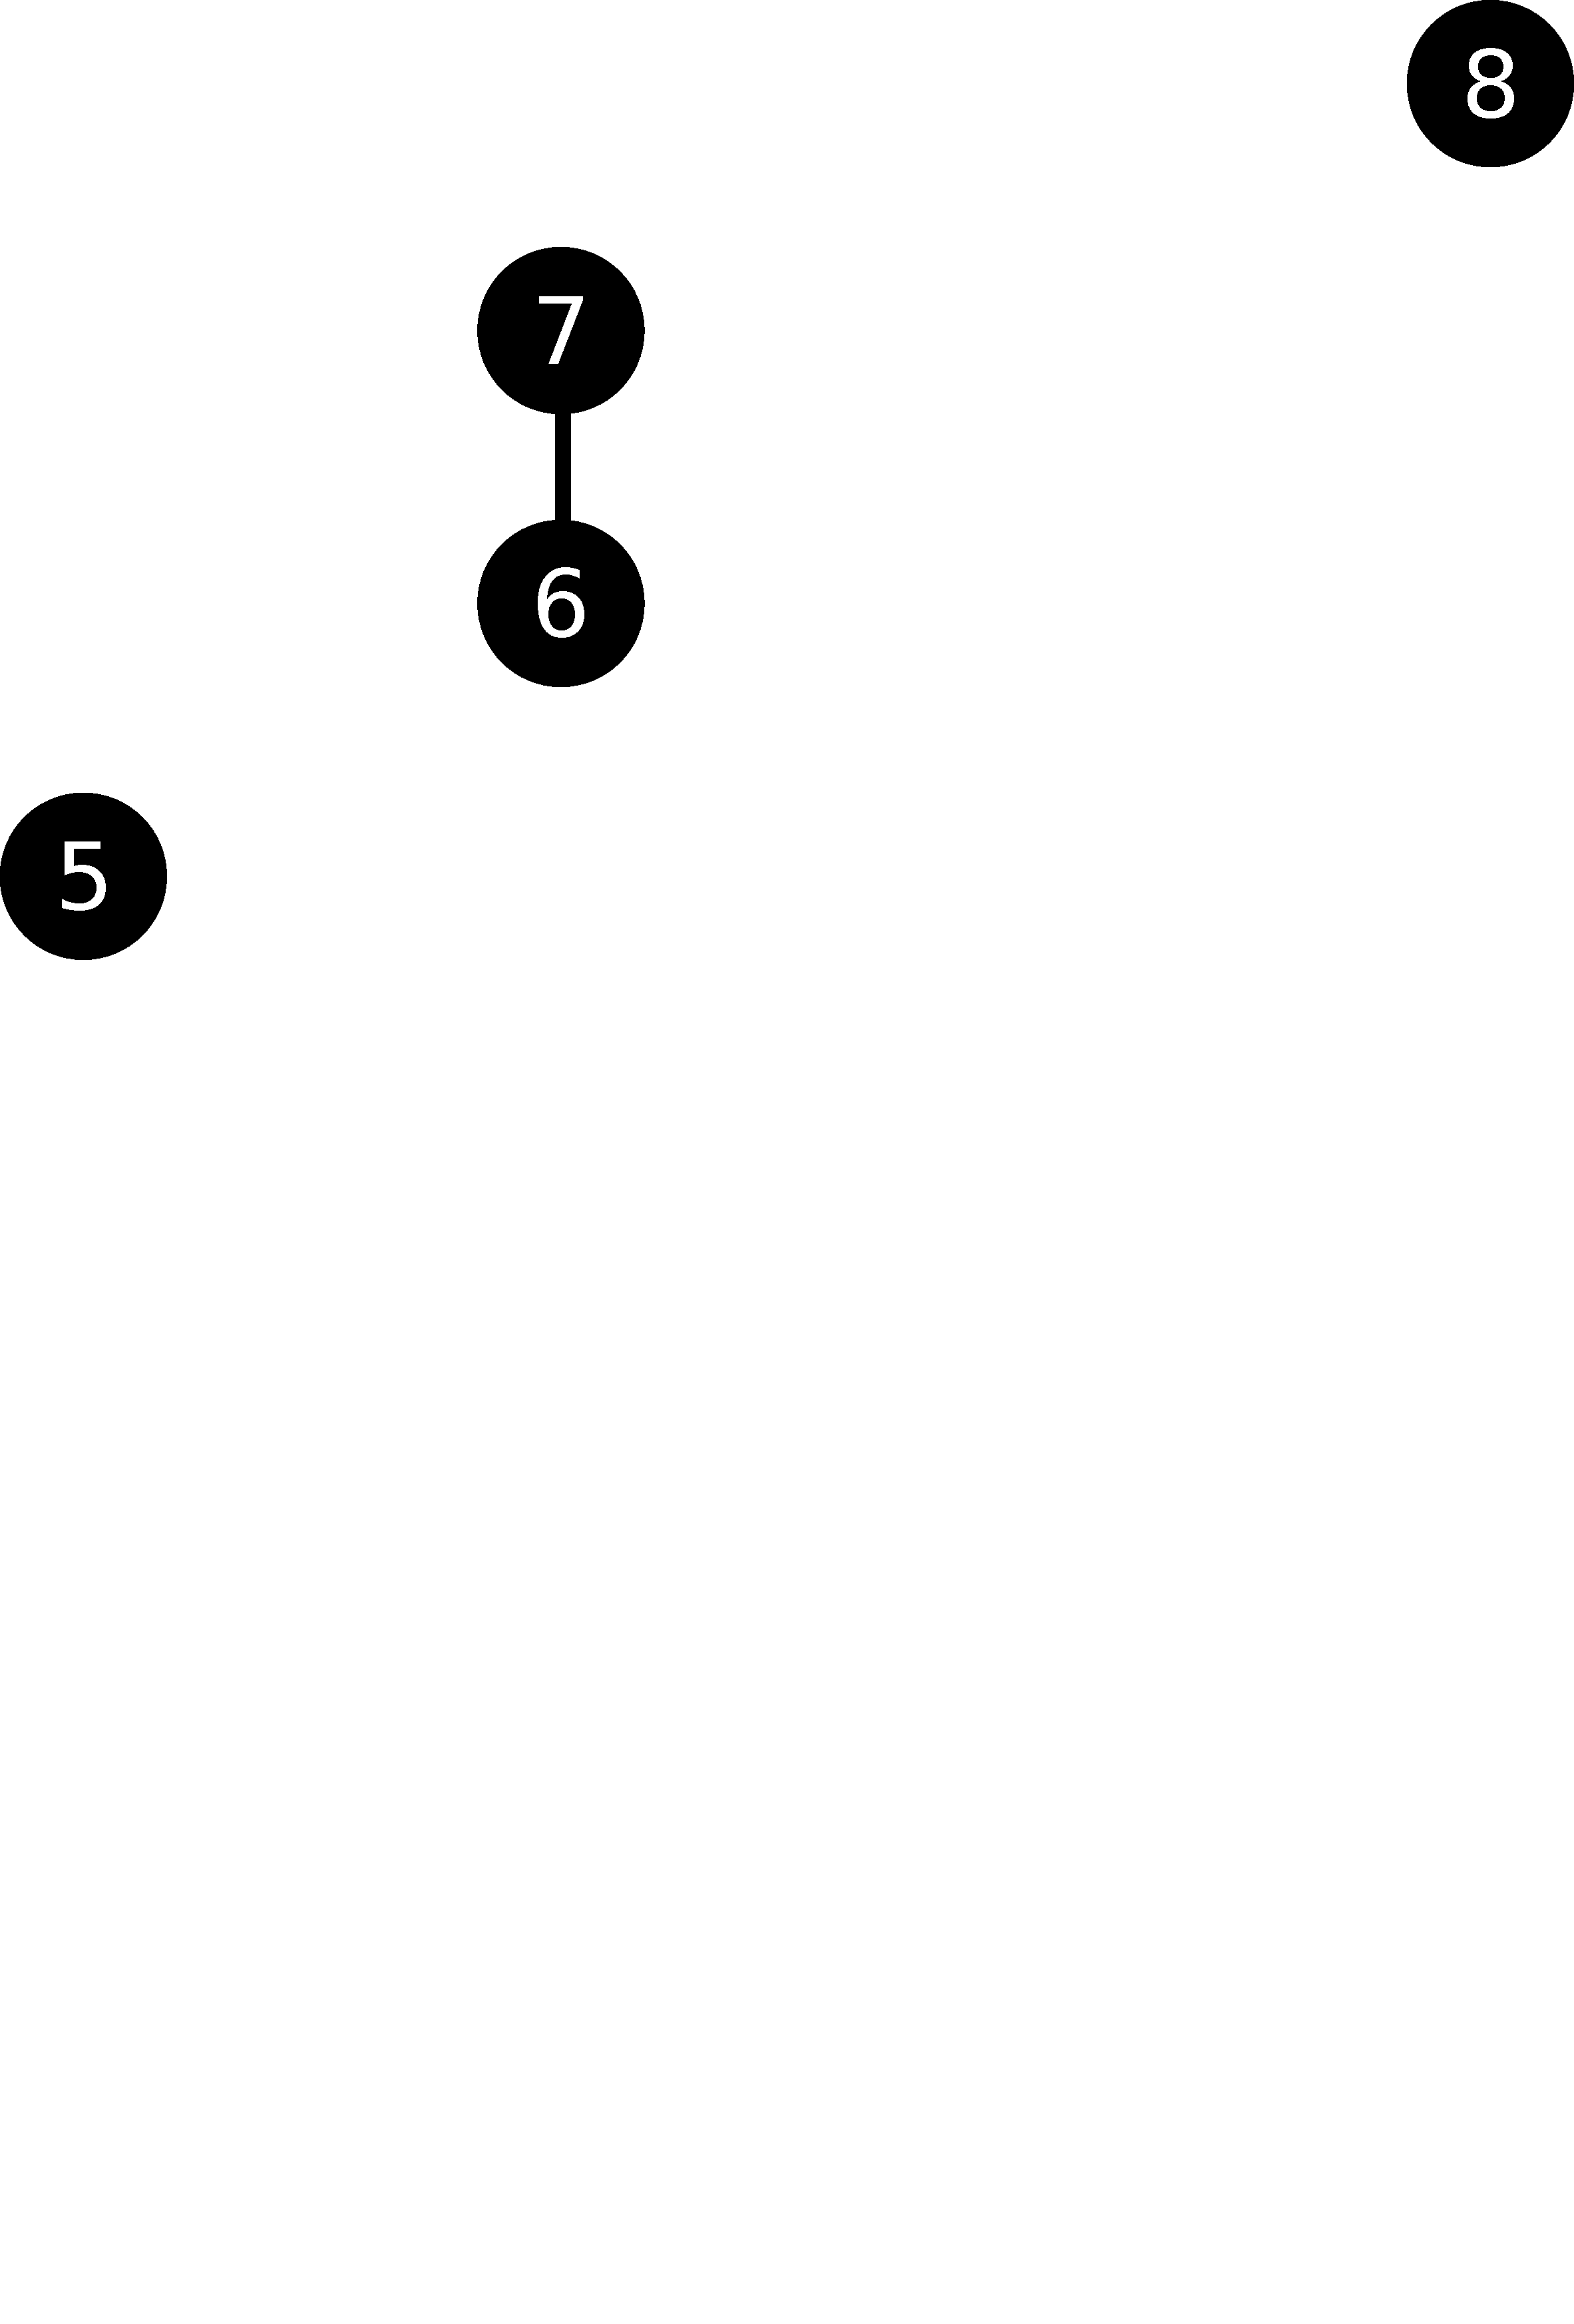
\includegraphics[scale=0.08]{./images/filtration/desc-tree/x4.pdf}}}%
    \qquad \qquad
    \subfloat[$CT(X)^5$]{{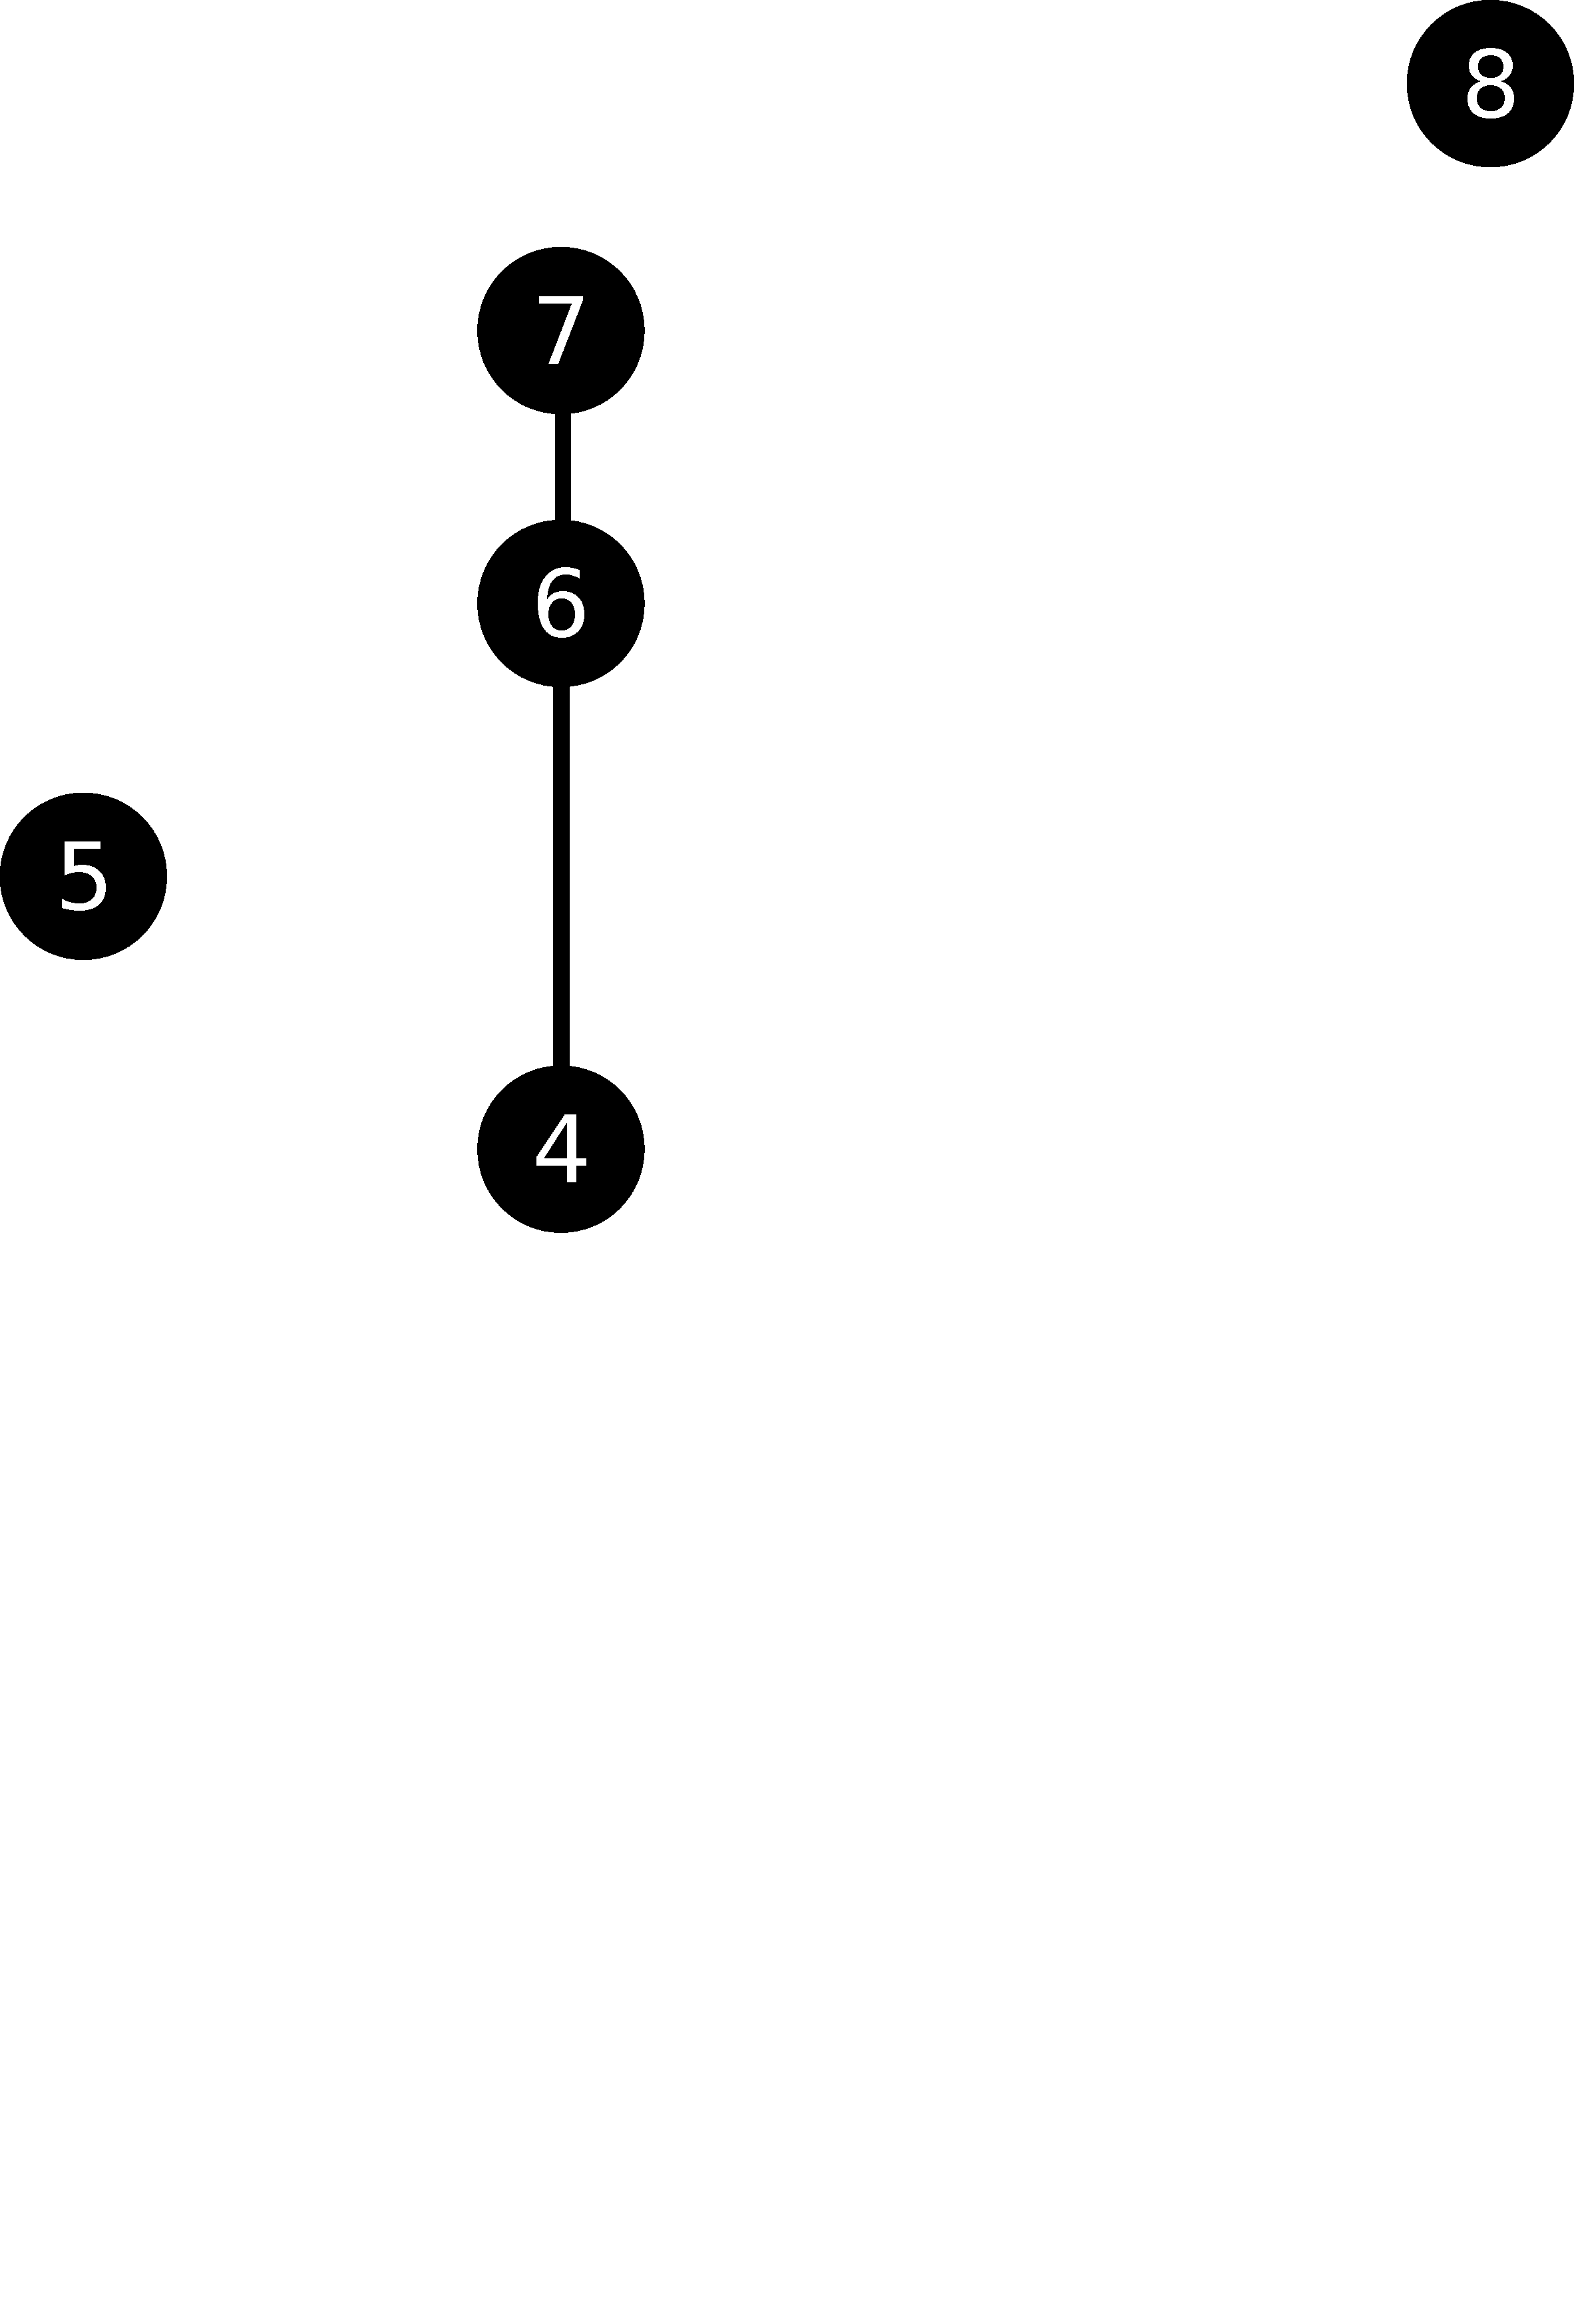
\includegraphics[scale=0.08]{./images/filtration/desc-tree/x5.pdf}}}%
    \qquad \qquad
    \subfloat[$CT(X)^4$]{{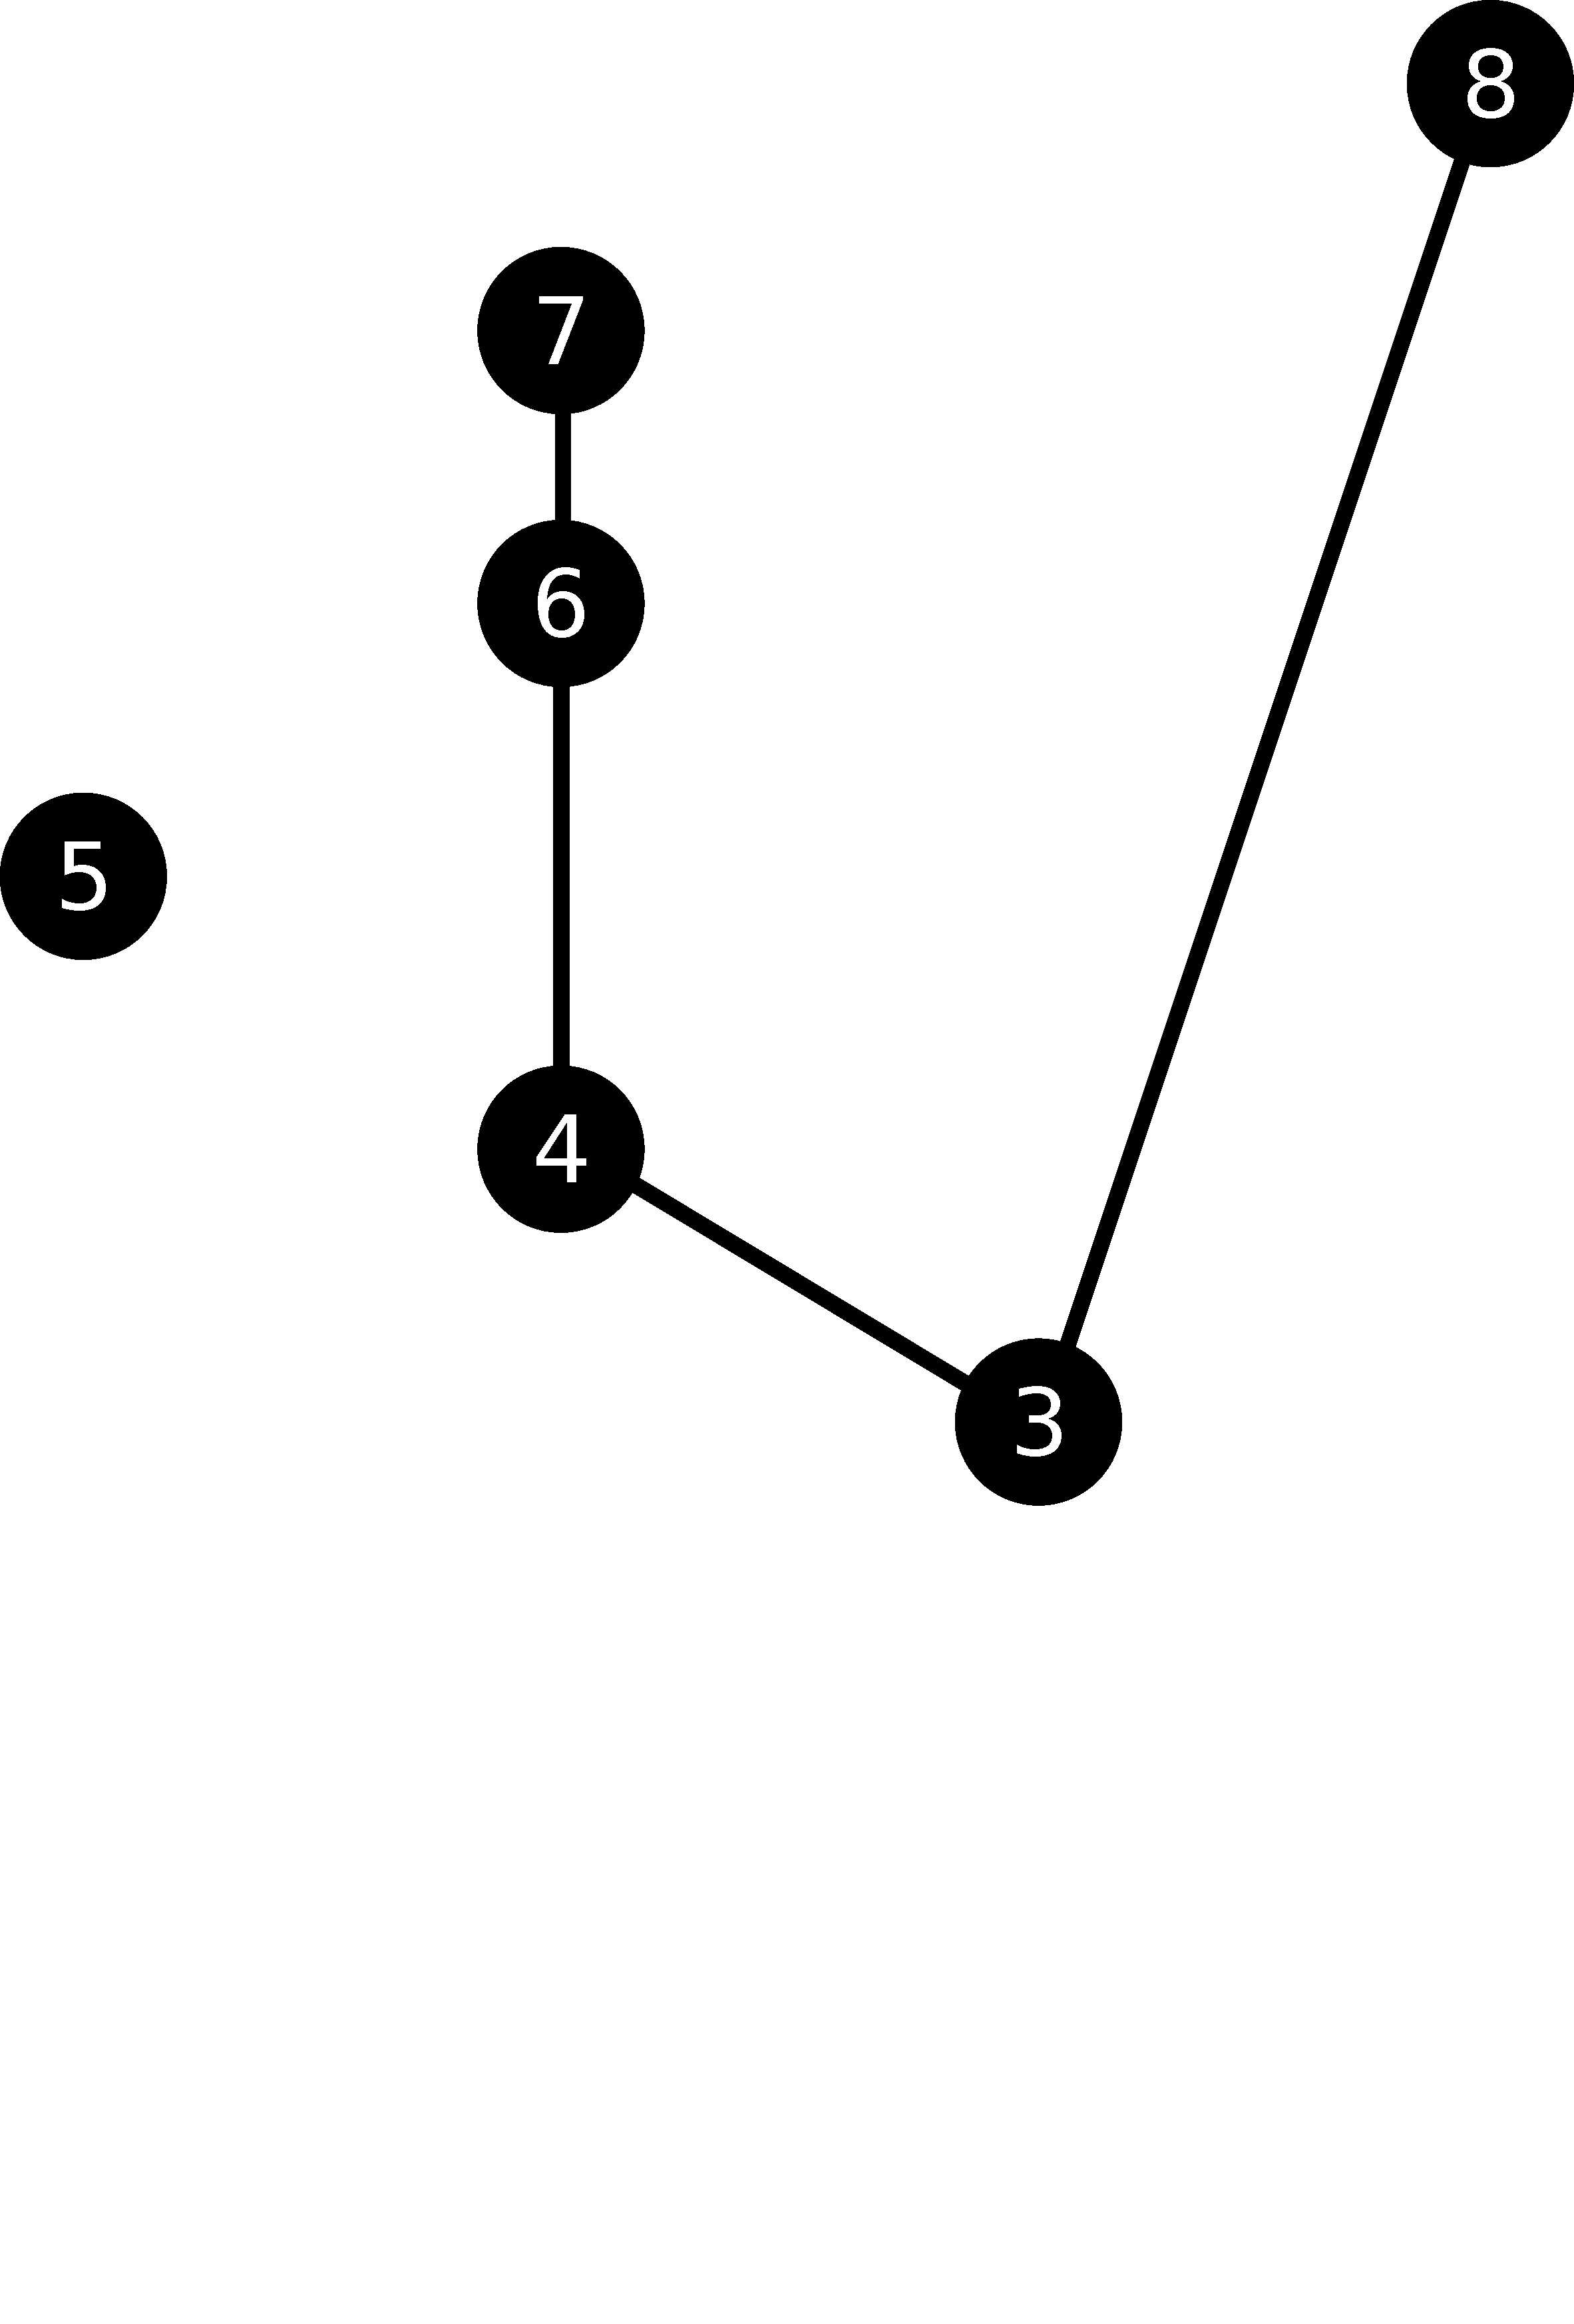
\includegraphics[scale=0.08]{./images/filtration/desc-tree/x6.pdf}}}%

    \par\bigskip

    \subfloat[$CT(X)^3$]{{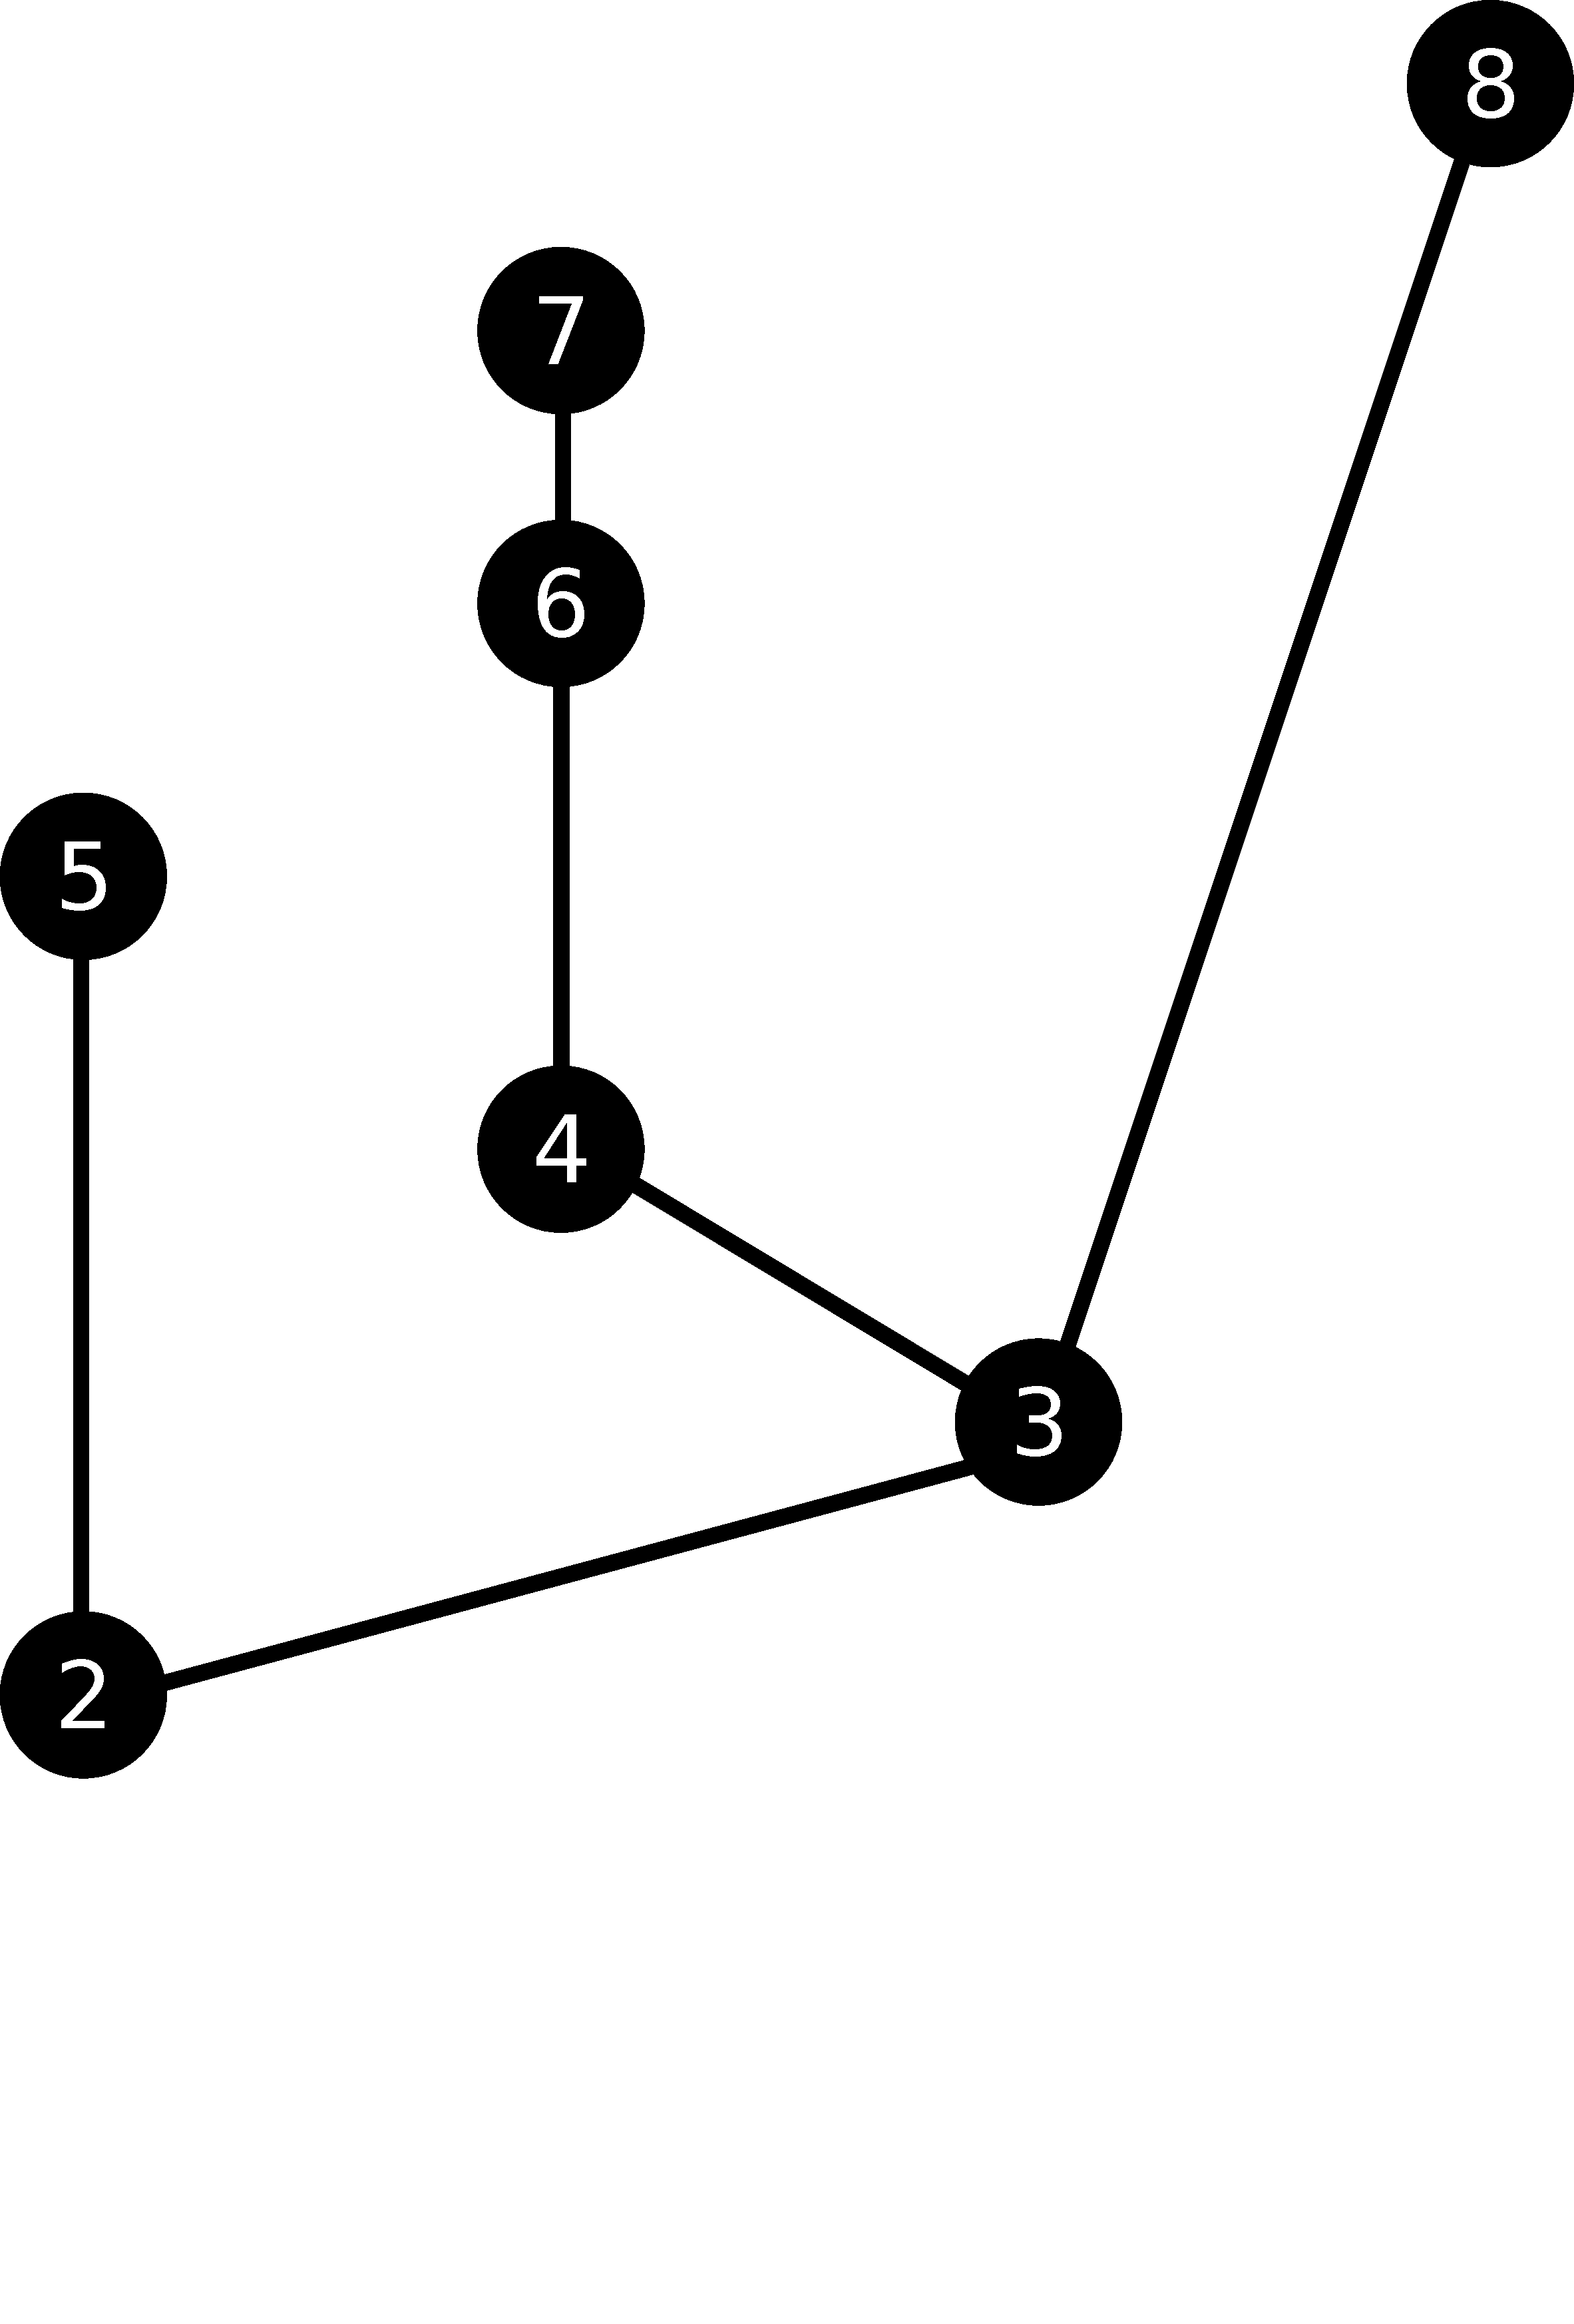
\includegraphics[scale=0.08]{./images/filtration/desc-tree/x7.pdf}}}%
    \qquad \qquad
    \subfloat[$CT(X)^2$]{{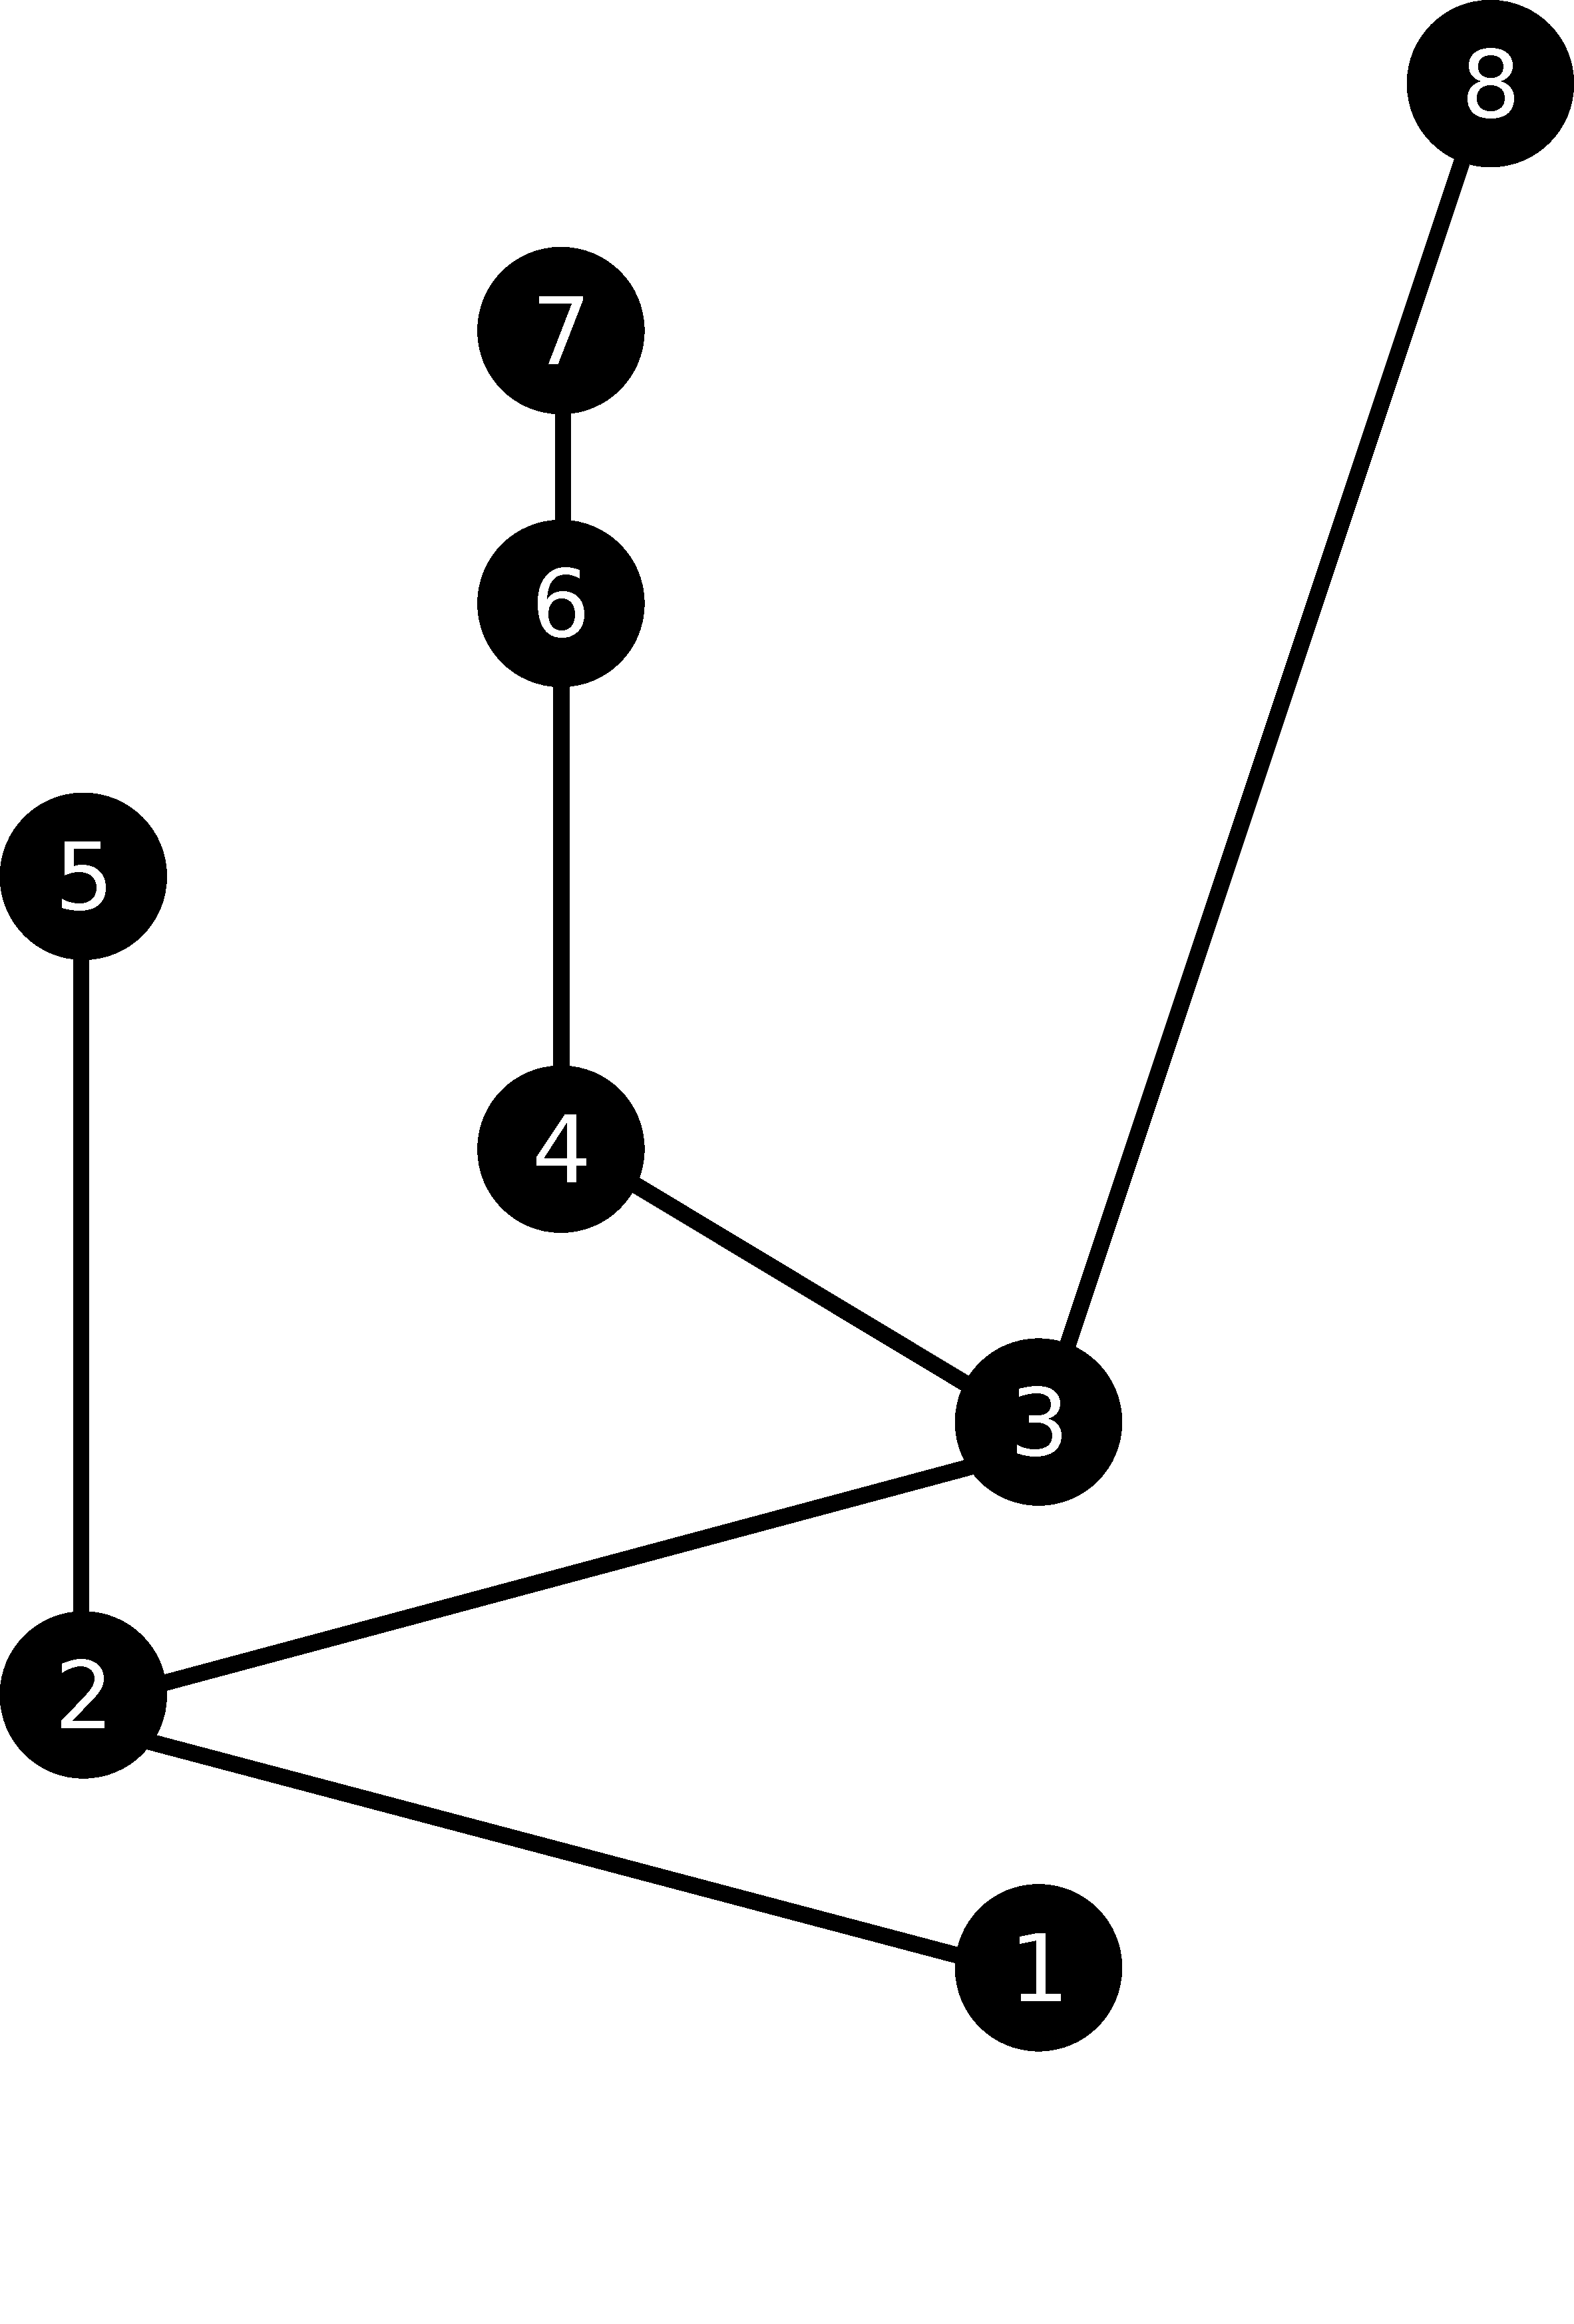
\includegraphics[scale=0.08]{./images/filtration/desc-tree/x8.pdf}}}%
    \qquad \qquad
    \subfloat[$CT(X)^1$]{{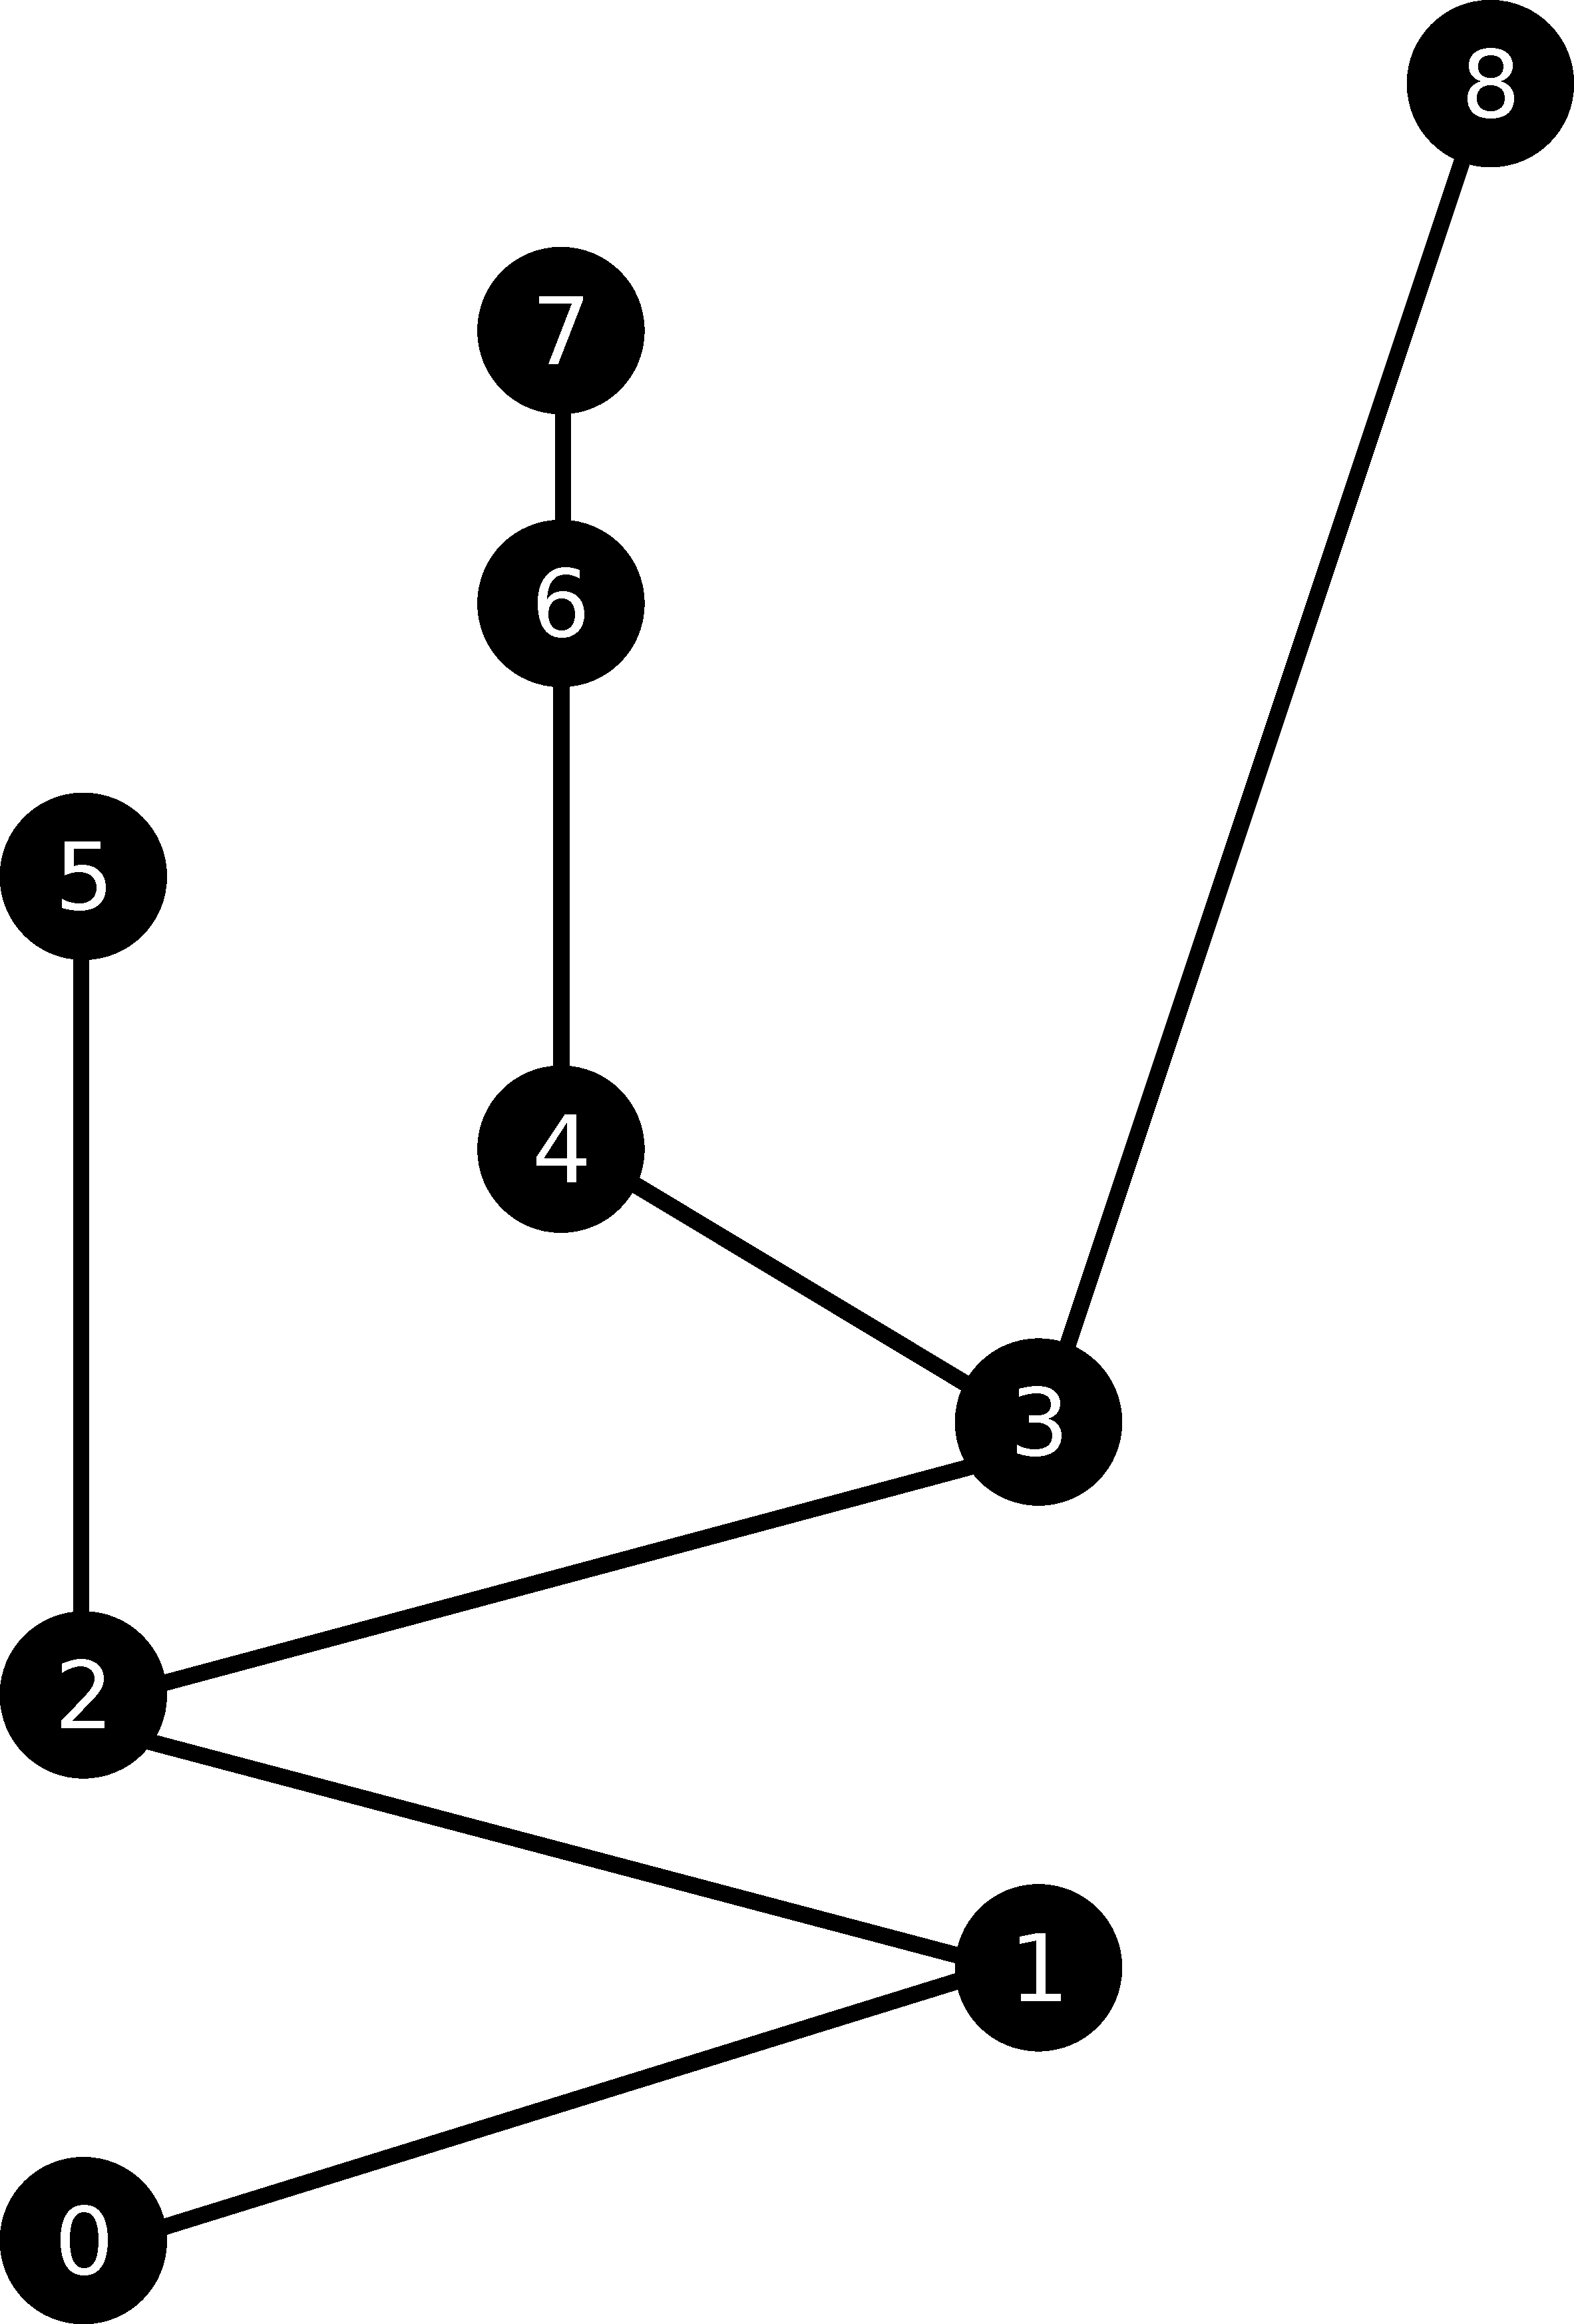
\includegraphics[scale=0.08]{./images/filtration/desc-tree/x9.pdf}}}%

    \caption{Descending filtration of the contour tree from Figure \ref{fig:mesh-join-split-contour} b.}%
    \label{fig:desc-filtration-tree}%
\end{figure}

\chapter{Additional Proofs}
\label{chapter-proofs}

\begin{lem} In a tree with no vertices of degree two at least half of the vertices are leaves. \end{lem}

\begin{proof}
    Let $T = (V, E)$ be a tree with no vertices of degree two and let $L \subseteq V$ be the set of all leaves. As all leaves have degree one we have that $L = \{u \in V: d(u) = 1\}$. Furthermore for any tree we know that $|E| = |V| - 1$. Let us now use the handshake lemma:

    $$ \sum_{u \in V}{d(u)} = 2|E| = 2(|V| - 1) = 2|V| - 2.$$

    We will not separe the sum on the leftmost hand side of the equation in two parts. One for the vertices vertices in $L$ and one for the vertices in $V\textbackslash L$.


    $$ \sum_{u \in L}{d(u)} + \sum_{u \in V\textbackslash L}{d(u)} = 2|V| - 2.$$

    All the vertices in $L$ are leaves. By definition the degree of a leaf is one. Therefore $\sum_{u \in L}{d(u)} = |L|$. This leads us to the following:

    $$  |L| + \sum_{u \in V\textbackslash L}{d(u)} = 2|V| - 2$$
    $$  |L|  = 2|V| - 2 - \sum_{u \in V\textbackslash L}{d(u)}.$$

    There are no vertices in $T$ of degree two and all vertices of degree one are in $L$. This means that all vertices in $V \textbackslash T$ have degree at least three. We can conclude that:
    $$\sum_{u \in V\textbackslash L}{d(u)} \ge \delta(T - L).|V\textbackslash L| = 3(|V| - |L|) $$

    Combining this with the previous equation we obtain that:

    $$  |L| \le 2|V| - 2 - 3(|V| - |L|)$$
    $$  |L| \le 2|V| - 2 - 3|V| + 3|L|$$
    $$  -2|L| \le -|V| - 2$$
    $$  |L| \ge \frac{|V|}{2} + 1$$

    Which is exactly what we set out to proove.


\end{proof}
%
% \begin{lem} There are at least $k$ vertices for every vertex of degree $k$ in a tree. \end{lem}
%
% \begin{proof}
%     Let $T$ be a tree and $u \in V(T)$ be a vertex in it. As any tree can be rooted, let us root $T$ at $u$ and call the new directed tree $T_u$. Let $U = \{u_1, u_2, ..., u_k\}$ be the neighbours of $u$. For each $u_i \in U$ if $u_i$ is not a leaf let $u_i$ be one of it's children. Repeat this process until every $u_i$ is a leaf. This is possible because $T$ is finite. All of the $u_i$ are distinct, for otherwise there would be a cycle in $T$.
%
% \end{proof}
%
%
% \chapter{Vector Spaces, Quiver Diagrams and Barcode Diagrams}
%
% *This chapter will probably be redistributed in the homology chapter. I'll probably remove it.*
%
% Should I define a vector space, bases, etc.?
%
% Should I define a vector space, bases, etc.?
%
%
% %Suppose we have a number of vector spaces with linear maps between con
% Suppose we have a number of vector spaces $(V_1, V_2, ...,V_n)$
%
% Suppose we have a number of vector spaces $(V_1, V_2, ...,V_n)$ together with linear maps $(f_1, f_2, ...,f_{n-1})$ that that map between consecutive vector spaces like follows : $f_i: V_i \to V_{i+1}, \forall i = 1, 2, ..., n -1$.
%
% A quiver representation is a directed multigraph where the vertices are sets and directed edges are function between sets. In our case the vertices will be vector spaces and the edges linear maps. The quiver diagram of the configuration we just described looks as follows:
%
% $$V_1 \overset{f_1}{\longrightarrow} V_2 \overset{f_2}{\longrightarrow} ... \overset{f_{n-1}}{\longrightarrow} V_n  $$
%
%
% "This sounds weird, fix it."
% Not that we can always extend any sequence of vector spaces with the null vector space and the null maps as follows:
%
% $$ 0 \longrightarrow ... \longrightarrow 0 \longrightarrow V_1 \overset{f_1}{\longrightarrow} V_2 \overset{f_2}{\longrightarrow} ... \overset{f_{n-1}}{\longrightarrow} V_n  \longrightarrow 0 \longrightarrow ... \longrightarrow 0$$
%
% A barcode diagram is a digram that shows which shows how the basis elements of the vector spaces evolve as they get mapped through the linear functions once we commit to particular basis elements for each vector space.
%
% Show a barcode diagram.
%
% A Chain Complex is a quiver representation where the image of each maps is a subset of the kernel of the next one.
%
% $$ ... \longrightarrow V_1 \overset{d_1}{\longrightarrow} V_2 \overset{d_2}{\longrightarrow} ... \overset{d_{n-1}}{\longrightarrow} V_n  \longrightarrow ... $$
%
% This example is a chain complex when $im(d_k) \subseteq ker(d_{k+1})$. As the image is a subset of the kernel the we can equivalently write this as the composition $d_{k+1}d_k = 0$. In practical terms once we commit to baseis multiplying consecutive matricies will equal the zero matrix. An important property of the barcode diagram of chain complexes is that no line can be longer than two units!
%
%
% \begin{ex}  A Simple Chain Complex \end{ex}
% Let us now for simplicity and demonstrational purposes assume that each $V_i$ is isomorphic to $\mathbb{R}^n$ for some $n \in \mathbb{Z}$.
%
%
% % @TODO Continue this.
% An exact sequence is a chain complex where $im(d_k) = ker(d_{k+1})$. Exact sequences are useful because of the nice properties like ...
%
% The homology of a chain complex is defined as a quantifier of how far a chain complex is from being an exact sequence. It is defined as: $ H_k = ker(d_{k+1}) / im(d_k) $
%
% Let $V$ be a vector space and $W$ a subspace of $V$. A coset of $W$ is the set $v + W = \{v + w : w \in W\}$.
%
% A quotient in a vector space is defined in the following way:
%
% $$ V/W = \{v + W: v \in V\} = \{\{v + w : w \in W\} : v \in V \}$$
%
% Show a picture of the cosets.
%
% Luckily in $\mathbb{R}^n$ we have the following theorem: $\mathbb{R}^n / \mathbb{R}^m \simeq \mathbb{R}^{n - m} $ where we have slightly abused notation as $\mathbb{R}^m$ can not be a subspace of $\mathbb{R}^n$, but we consider it isomorhpic to one for $m \le n$.
%
% $$ \mathbb{R}^3 {\longrightarrow} \mathbb{R}^2 {\longrightarrow} \mathbb{R}^4 $$
%
%
%
%
% \chapter{External Material}
% \lipsum[3-3]
% \chapter{Ethical Issues Addressed}
%
% \chapter{Topologies on $\mathbb{R}$ and $\mathbb{R}^n$}
%
% \begin{ex} The standard topologly on $\mathbb{R}$.  \end{ex}
%
% The standard topology on $\mathbb{R}$ is build from subsets of $\mathbb{R}$ called open balls. The open ball centered at $x \in \mathbb{R}$ with radius $\epsilon \in \mathbb{R}^+$ is a subset $B_\epsilon(x)$ of $\mathbb{R}$ defined as:
%
% $$ B_\epsilon(x) = \{y \in \mathbb{R} : |x - y| < \epsilon \} .$$
%
% These are all the points whose distance from $x$ is less than $\epsilon$. The collection of all open balls as $x$ ranges over $\mathbb{R}$ and $\epsilon$ ranges over $\mathbb{R}^+$ makes up the building blocks of the topology. The open sets in the topology are all the open balls together with their arbitrary unions and finite intersections.
%
%
% \begin{ex} The standard topologly on $\mathbb{R}^n$.  \end{ex}
%
% We can slightly adjust the previous definition to obtain a topology on $\mathbb{R}^n$. We just have to consider $\vec{x} \text{ and } \vec{y}$ to be vectors in $\mathbb{R}^n$ and evaluate the distance between them using the standard Eucledian metric. That is if $\vec{x} = (x_1, ..., x_n)$ and $\vec{y} = (y_1, ..., y_n)$ then:
%
% $$ B_\epsilon(\vec{x}) = \{\vec{y} \in \mathbb{R}^n : \sqrt{\sum_{i = 1}^{n}{(x_i - y_i) ^ 2}} < \epsilon \} $$
%
% is a subset of $\mathbb{R}^n$ with all points of distance less than $\epsilon$ from $\vec{x}$. Like previously the topology on $\mathbb{R}^n$ is obtained through arbitrary unions and finite intersections of the set of open balls.
%
%
%
% \chapter{Circle and Real Line}
%
% Consider for example the real line $\mathbb{R}$ and the circle $S^1$. There are differentiable functions from $\mathbb{R}$ to $\mathbb{R}$ such as $y = x$ which do not take a minimum or a maximum value. They can be arbitrary large or small on the manifold $\mathbb{R}$. It is not possible to define such a differentiable function from $S^1$ to $\mathbb{R}$. This is due to the maximum value theorem. More formally a differentiable function is continuous and $S^1$ is compact. By [] the continuous image of a compact space is compact and by [] the compact spaces of $\mathbb{R}$ are closed and bounded. Closed and bounded means unions of intervals of the form $[a, b]$ where $|a|, |b| < \epsilon$ for some $\epsilon \in \mathbb{R}$. We can pick the lower bound of the interval with the lowest lower bound and the upper bound of the interval with the highest upper bound for the minimum and maximum values. Therefore any differentiable function defined on $S^1$ will take a minimum and a maximum value.



\chapter{Github Repositories}
\label{chapter-github}


DP Algorithm - \url{https://github.com/famouscake/w-detector}

2xBFS Algorithm - \url{https://github.com/famouscake/w-detector}

Contour Tree Algoritm - \url{https://github.com/famouscake/ContourTree}


\chapter{Ethical Issues Addressed}
\label{chapter-ethical}

\section{Data Sources}

For this project data sources were required to compute contour trees. The data sources that were used are publicly available on the Internet. They did not require any special permissionssions to use.

\section{Software}
All software that was used is publicly available on the internet and free. It has been referenced and acknowledgement in the text.


\end{appendices}
